\documentclass{article}
\usepackage{graphicx, color}
\newcommand{\hlnumber}[1]{\textcolor[rgb]{0,0,0}{#1}}%
\newcommand{\hlfunctioncall}[1]{\textcolor[rgb]{.5,0,.33}{\textbf{#1}}}%
\newcommand{\hlstring}[1]{\textcolor[rgb]{.6,.6,1}{#1}}%
\newcommand{\hlkeyword}[1]{\textbf{#1}}%
\newcommand{\hlargument}[1]{\textcolor[rgb]{.69,.25,.02}{#1}}%
\newcommand{\hlcomment}[1]{\textcolor[rgb]{.18,.6,.34}{#1}}%
\newcommand{\hlroxygencomment}[1]{\textcolor[rgb]{.44,.48,.7}{#1}}%
\newcommand{\hlformalargs}[1]{\hlargument{#1}}%
\newcommand{\hleqformalargs}[1]{\hlargument{#1}}%
\newcommand{\hlassignement}[1]{\textbf{#1}}%
\newcommand{\hlpackage}[1]{\textcolor[rgb]{.59,.71,.145}{#1}}%
\newcommand{\hlslot}[1]{\textit{#1}}%
\newcommand{\hlsymbol}[1]{#1}%
\newcommand{\hlprompt}[1]{\textcolor[rgb]{.5,.5,.5}{#1}}%

\usepackage{color}%
 
\newsavebox{\hlnormalsizeboxclosebrace}%
\newsavebox{\hlnormalsizeboxopenbrace}%
\newsavebox{\hlnormalsizeboxbackslash}%
\newsavebox{\hlnormalsizeboxlessthan}%
\newsavebox{\hlnormalsizeboxgreaterthan}%
\newsavebox{\hlnormalsizeboxdollar}%
\newsavebox{\hlnormalsizeboxunderscore}%
\newsavebox{\hlnormalsizeboxand}%
\newsavebox{\hlnormalsizeboxhash}%
\newsavebox{\hlnormalsizeboxat}%
\newsavebox{\hlnormalsizeboxpercent}% 
\newsavebox{\hlnormalsizeboxhat}%
\newsavebox{\hlnormalsizeboxsinglequote}%
\newsavebox{\hlnormalsizeboxbacktick}%

\setbox\hlnormalsizeboxopenbrace=\hbox{\begin{normalsize}\verb.{.\end{normalsize}}%
\setbox\hlnormalsizeboxclosebrace=\hbox{\begin{normalsize}\verb.}.\end{normalsize}}%
\setbox\hlnormalsizeboxlessthan=\hbox{\begin{normalsize}\verb.<.\end{normalsize}}%
\setbox\hlnormalsizeboxdollar=\hbox{\begin{normalsize}\verb.$.\end{normalsize}}%
\setbox\hlnormalsizeboxunderscore=\hbox{\begin{normalsize}\verb._.\end{normalsize}}%
\setbox\hlnormalsizeboxand=\hbox{\begin{normalsize}\verb.&.\end{normalsize}}%
\setbox\hlnormalsizeboxhash=\hbox{\begin{normalsize}\verb.#.\end{normalsize}}%
\setbox\hlnormalsizeboxat=\hbox{\begin{normalsize}\verb.@.\end{normalsize}}%
\setbox\hlnormalsizeboxbackslash=\hbox{\begin{normalsize}\verb.\.\end{normalsize}}%
\setbox\hlnormalsizeboxgreaterthan=\hbox{\begin{normalsize}\verb.>.\end{normalsize}}%
\setbox\hlnormalsizeboxpercent=\hbox{\begin{normalsize}\verb.%.\end{normalsize}}%
\setbox\hlnormalsizeboxhat=\hbox{\begin{normalsize}\verb.^.\end{normalsize}}%
\setbox\hlnormalsizeboxsinglequote=\hbox{\begin{normalsize}\verb.'.\end{normalsize}}%
\setbox\hlnormalsizeboxbacktick=\hbox{\begin{normalsize}\verb.`.\end{normalsize}}%
\setbox\hlnormalsizeboxhat=\hbox{\begin{normalsize}\verb.^.\end{normalsize}}%



\newsavebox{\hltinyboxclosebrace}%
\newsavebox{\hltinyboxopenbrace}%
\newsavebox{\hltinyboxbackslash}%
\newsavebox{\hltinyboxlessthan}%
\newsavebox{\hltinyboxgreaterthan}%
\newsavebox{\hltinyboxdollar}%
\newsavebox{\hltinyboxunderscore}%
\newsavebox{\hltinyboxand}%
\newsavebox{\hltinyboxhash}%
\newsavebox{\hltinyboxat}%
\newsavebox{\hltinyboxpercent}% 
\newsavebox{\hltinyboxhat}%
\newsavebox{\hltinyboxsinglequote}%
\newsavebox{\hltinyboxbacktick}%

\setbox\hltinyboxopenbrace=\hbox{\begin{tiny}\verb.{.\end{tiny}}%
\setbox\hltinyboxclosebrace=\hbox{\begin{tiny}\verb.}.\end{tiny}}%
\setbox\hltinyboxlessthan=\hbox{\begin{tiny}\verb.<.\end{tiny}}%
\setbox\hltinyboxdollar=\hbox{\begin{tiny}\verb.$.\end{tiny}}%
\setbox\hltinyboxunderscore=\hbox{\begin{tiny}\verb._.\end{tiny}}%
\setbox\hltinyboxand=\hbox{\begin{tiny}\verb.&.\end{tiny}}%
\setbox\hltinyboxhash=\hbox{\begin{tiny}\verb.#.\end{tiny}}%
\setbox\hltinyboxat=\hbox{\begin{tiny}\verb.@.\end{tiny}}%
\setbox\hltinyboxbackslash=\hbox{\begin{tiny}\verb.\.\end{tiny}}%
\setbox\hltinyboxgreaterthan=\hbox{\begin{tiny}\verb.>.\end{tiny}}%
\setbox\hltinyboxpercent=\hbox{\begin{tiny}\verb.%.\end{tiny}}%
\setbox\hltinyboxhat=\hbox{\begin{tiny}\verb.^.\end{tiny}}%
\setbox\hltinyboxsinglequote=\hbox{\begin{tiny}\verb.'.\end{tiny}}%
\setbox\hltinyboxbacktick=\hbox{\begin{tiny}\verb.`.\end{tiny}}%
\setbox\hltinyboxhat=\hbox{\begin{tiny}\verb.^.\end{tiny}}%



\newsavebox{\hlscriptsizeboxclosebrace}%
\newsavebox{\hlscriptsizeboxopenbrace}%
\newsavebox{\hlscriptsizeboxbackslash}%
\newsavebox{\hlscriptsizeboxlessthan}%
\newsavebox{\hlscriptsizeboxgreaterthan}%
\newsavebox{\hlscriptsizeboxdollar}%
\newsavebox{\hlscriptsizeboxunderscore}%
\newsavebox{\hlscriptsizeboxand}%
\newsavebox{\hlscriptsizeboxhash}%
\newsavebox{\hlscriptsizeboxat}%
\newsavebox{\hlscriptsizeboxpercent}% 
\newsavebox{\hlscriptsizeboxhat}%
\newsavebox{\hlscriptsizeboxsinglequote}%
\newsavebox{\hlscriptsizeboxbacktick}%

\setbox\hlscriptsizeboxopenbrace=\hbox{\begin{scriptsize}\verb.{.\end{scriptsize}}%
\setbox\hlscriptsizeboxclosebrace=\hbox{\begin{scriptsize}\verb.}.\end{scriptsize}}%
\setbox\hlscriptsizeboxlessthan=\hbox{\begin{scriptsize}\verb.<.\end{scriptsize}}%
\setbox\hlscriptsizeboxdollar=\hbox{\begin{scriptsize}\verb.$.\end{scriptsize}}%
\setbox\hlscriptsizeboxunderscore=\hbox{\begin{scriptsize}\verb._.\end{scriptsize}}%
\setbox\hlscriptsizeboxand=\hbox{\begin{scriptsize}\verb.&.\end{scriptsize}}%
\setbox\hlscriptsizeboxhash=\hbox{\begin{scriptsize}\verb.#.\end{scriptsize}}%
\setbox\hlscriptsizeboxat=\hbox{\begin{scriptsize}\verb.@.\end{scriptsize}}%
\setbox\hlscriptsizeboxbackslash=\hbox{\begin{scriptsize}\verb.\.\end{scriptsize}}%
\setbox\hlscriptsizeboxgreaterthan=\hbox{\begin{scriptsize}\verb.>.\end{scriptsize}}%
\setbox\hlscriptsizeboxpercent=\hbox{\begin{scriptsize}\verb.%.\end{scriptsize}}%
\setbox\hlscriptsizeboxhat=\hbox{\begin{scriptsize}\verb.^.\end{scriptsize}}%
\setbox\hlscriptsizeboxsinglequote=\hbox{\begin{scriptsize}\verb.'.\end{scriptsize}}%
\setbox\hlscriptsizeboxbacktick=\hbox{\begin{scriptsize}\verb.`.\end{scriptsize}}%
\setbox\hlscriptsizeboxhat=\hbox{\begin{scriptsize}\verb.^.\end{scriptsize}}%



\newsavebox{\hlfootnotesizeboxclosebrace}%
\newsavebox{\hlfootnotesizeboxopenbrace}%
\newsavebox{\hlfootnotesizeboxbackslash}%
\newsavebox{\hlfootnotesizeboxlessthan}%
\newsavebox{\hlfootnotesizeboxgreaterthan}%
\newsavebox{\hlfootnotesizeboxdollar}%
\newsavebox{\hlfootnotesizeboxunderscore}%
\newsavebox{\hlfootnotesizeboxand}%
\newsavebox{\hlfootnotesizeboxhash}%
\newsavebox{\hlfootnotesizeboxat}%
\newsavebox{\hlfootnotesizeboxpercent}% 
\newsavebox{\hlfootnotesizeboxhat}%
\newsavebox{\hlfootnotesizeboxsinglequote}%
\newsavebox{\hlfootnotesizeboxbacktick}%

\setbox\hlfootnotesizeboxopenbrace=\hbox{\begin{footnotesize}\verb.{.\end{footnotesize}}%
\setbox\hlfootnotesizeboxclosebrace=\hbox{\begin{footnotesize}\verb.}.\end{footnotesize}}%
\setbox\hlfootnotesizeboxlessthan=\hbox{\begin{footnotesize}\verb.<.\end{footnotesize}}%
\setbox\hlfootnotesizeboxdollar=\hbox{\begin{footnotesize}\verb.$.\end{footnotesize}}%
\setbox\hlfootnotesizeboxunderscore=\hbox{\begin{footnotesize}\verb._.\end{footnotesize}}%
\setbox\hlfootnotesizeboxand=\hbox{\begin{footnotesize}\verb.&.\end{footnotesize}}%
\setbox\hlfootnotesizeboxhash=\hbox{\begin{footnotesize}\verb.#.\end{footnotesize}}%
\setbox\hlfootnotesizeboxat=\hbox{\begin{footnotesize}\verb.@.\end{footnotesize}}%
\setbox\hlfootnotesizeboxbackslash=\hbox{\begin{footnotesize}\verb.\.\end{footnotesize}}%
\setbox\hlfootnotesizeboxgreaterthan=\hbox{\begin{footnotesize}\verb.>.\end{footnotesize}}%
\setbox\hlfootnotesizeboxpercent=\hbox{\begin{footnotesize}\verb.%.\end{footnotesize}}%
\setbox\hlfootnotesizeboxhat=\hbox{\begin{footnotesize}\verb.^.\end{footnotesize}}%
\setbox\hlfootnotesizeboxsinglequote=\hbox{\begin{footnotesize}\verb.'.\end{footnotesize}}%
\setbox\hlfootnotesizeboxbacktick=\hbox{\begin{footnotesize}\verb.`.\end{footnotesize}}%
\setbox\hlfootnotesizeboxhat=\hbox{\begin{footnotesize}\verb.^.\end{footnotesize}}%



\newsavebox{\hlsmallboxclosebrace}%
\newsavebox{\hlsmallboxopenbrace}%
\newsavebox{\hlsmallboxbackslash}%
\newsavebox{\hlsmallboxlessthan}%
\newsavebox{\hlsmallboxgreaterthan}%
\newsavebox{\hlsmallboxdollar}%
\newsavebox{\hlsmallboxunderscore}%
\newsavebox{\hlsmallboxand}%
\newsavebox{\hlsmallboxhash}%
\newsavebox{\hlsmallboxat}%
\newsavebox{\hlsmallboxpercent}% 
\newsavebox{\hlsmallboxhat}%
\newsavebox{\hlsmallboxsinglequote}%
\newsavebox{\hlsmallboxbacktick}%

\setbox\hlsmallboxopenbrace=\hbox{\begin{small}\verb.{.\end{small}}%
\setbox\hlsmallboxclosebrace=\hbox{\begin{small}\verb.}.\end{small}}%
\setbox\hlsmallboxlessthan=\hbox{\begin{small}\verb.<.\end{small}}%
\setbox\hlsmallboxdollar=\hbox{\begin{small}\verb.$.\end{small}}%
\setbox\hlsmallboxunderscore=\hbox{\begin{small}\verb._.\end{small}}%
\setbox\hlsmallboxand=\hbox{\begin{small}\verb.&.\end{small}}%
\setbox\hlsmallboxhash=\hbox{\begin{small}\verb.#.\end{small}}%
\setbox\hlsmallboxat=\hbox{\begin{small}\verb.@.\end{small}}%
\setbox\hlsmallboxbackslash=\hbox{\begin{small}\verb.\.\end{small}}%
\setbox\hlsmallboxgreaterthan=\hbox{\begin{small}\verb.>.\end{small}}%
\setbox\hlsmallboxpercent=\hbox{\begin{small}\verb.%.\end{small}}%
\setbox\hlsmallboxhat=\hbox{\begin{small}\verb.^.\end{small}}%
\setbox\hlsmallboxsinglequote=\hbox{\begin{small}\verb.'.\end{small}}%
\setbox\hlsmallboxbacktick=\hbox{\begin{small}\verb.`.\end{small}}%
\setbox\hlsmallboxhat=\hbox{\begin{small}\verb.^.\end{small}}%



\newsavebox{\hllargeboxclosebrace}%
\newsavebox{\hllargeboxopenbrace}%
\newsavebox{\hllargeboxbackslash}%
\newsavebox{\hllargeboxlessthan}%
\newsavebox{\hllargeboxgreaterthan}%
\newsavebox{\hllargeboxdollar}%
\newsavebox{\hllargeboxunderscore}%
\newsavebox{\hllargeboxand}%
\newsavebox{\hllargeboxhash}%
\newsavebox{\hllargeboxat}%
\newsavebox{\hllargeboxpercent}% 
\newsavebox{\hllargeboxhat}%
\newsavebox{\hllargeboxsinglequote}%
\newsavebox{\hllargeboxbacktick}%

\setbox\hllargeboxopenbrace=\hbox{\begin{large}\verb.{.\end{large}}%
\setbox\hllargeboxclosebrace=\hbox{\begin{large}\verb.}.\end{large}}%
\setbox\hllargeboxlessthan=\hbox{\begin{large}\verb.<.\end{large}}%
\setbox\hllargeboxdollar=\hbox{\begin{large}\verb.$.\end{large}}%
\setbox\hllargeboxunderscore=\hbox{\begin{large}\verb._.\end{large}}%
\setbox\hllargeboxand=\hbox{\begin{large}\verb.&.\end{large}}%
\setbox\hllargeboxhash=\hbox{\begin{large}\verb.#.\end{large}}%
\setbox\hllargeboxat=\hbox{\begin{large}\verb.@.\end{large}}%
\setbox\hllargeboxbackslash=\hbox{\begin{large}\verb.\.\end{large}}%
\setbox\hllargeboxgreaterthan=\hbox{\begin{large}\verb.>.\end{large}}%
\setbox\hllargeboxpercent=\hbox{\begin{large}\verb.%.\end{large}}%
\setbox\hllargeboxhat=\hbox{\begin{large}\verb.^.\end{large}}%
\setbox\hllargeboxsinglequote=\hbox{\begin{large}\verb.'.\end{large}}%
\setbox\hllargeboxbacktick=\hbox{\begin{large}\verb.`.\end{large}}%
\setbox\hllargeboxhat=\hbox{\begin{large}\verb.^.\end{large}}%



\newsavebox{\hlLargeboxclosebrace}%
\newsavebox{\hlLargeboxopenbrace}%
\newsavebox{\hlLargeboxbackslash}%
\newsavebox{\hlLargeboxlessthan}%
\newsavebox{\hlLargeboxgreaterthan}%
\newsavebox{\hlLargeboxdollar}%
\newsavebox{\hlLargeboxunderscore}%
\newsavebox{\hlLargeboxand}%
\newsavebox{\hlLargeboxhash}%
\newsavebox{\hlLargeboxat}%
\newsavebox{\hlLargeboxpercent}% 
\newsavebox{\hlLargeboxhat}%
\newsavebox{\hlLargeboxsinglequote}%
\newsavebox{\hlLargeboxbacktick}%

\setbox\hlLargeboxopenbrace=\hbox{\begin{Large}\verb.{.\end{Large}}%
\setbox\hlLargeboxclosebrace=\hbox{\begin{Large}\verb.}.\end{Large}}%
\setbox\hlLargeboxlessthan=\hbox{\begin{Large}\verb.<.\end{Large}}%
\setbox\hlLargeboxdollar=\hbox{\begin{Large}\verb.$.\end{Large}}%
\setbox\hlLargeboxunderscore=\hbox{\begin{Large}\verb._.\end{Large}}%
\setbox\hlLargeboxand=\hbox{\begin{Large}\verb.&.\end{Large}}%
\setbox\hlLargeboxhash=\hbox{\begin{Large}\verb.#.\end{Large}}%
\setbox\hlLargeboxat=\hbox{\begin{Large}\verb.@.\end{Large}}%
\setbox\hlLargeboxbackslash=\hbox{\begin{Large}\verb.\.\end{Large}}%
\setbox\hlLargeboxgreaterthan=\hbox{\begin{Large}\verb.>.\end{Large}}%
\setbox\hlLargeboxpercent=\hbox{\begin{Large}\verb.%.\end{Large}}%
\setbox\hlLargeboxhat=\hbox{\begin{Large}\verb.^.\end{Large}}%
\setbox\hlLargeboxsinglequote=\hbox{\begin{Large}\verb.'.\end{Large}}%
\setbox\hlLargeboxbacktick=\hbox{\begin{Large}\verb.`.\end{Large}}%
\setbox\hlLargeboxhat=\hbox{\begin{Large}\verb.^.\end{Large}}%



\newsavebox{\hlLARGEboxclosebrace}%
\newsavebox{\hlLARGEboxopenbrace}%
\newsavebox{\hlLARGEboxbackslash}%
\newsavebox{\hlLARGEboxlessthan}%
\newsavebox{\hlLARGEboxgreaterthan}%
\newsavebox{\hlLARGEboxdollar}%
\newsavebox{\hlLARGEboxunderscore}%
\newsavebox{\hlLARGEboxand}%
\newsavebox{\hlLARGEboxhash}%
\newsavebox{\hlLARGEboxat}%
\newsavebox{\hlLARGEboxpercent}% 
\newsavebox{\hlLARGEboxhat}%
\newsavebox{\hlLARGEboxsinglequote}%
\newsavebox{\hlLARGEboxbacktick}%

\setbox\hlLARGEboxopenbrace=\hbox{\begin{LARGE}\verb.{.\end{LARGE}}%
\setbox\hlLARGEboxclosebrace=\hbox{\begin{LARGE}\verb.}.\end{LARGE}}%
\setbox\hlLARGEboxlessthan=\hbox{\begin{LARGE}\verb.<.\end{LARGE}}%
\setbox\hlLARGEboxdollar=\hbox{\begin{LARGE}\verb.$.\end{LARGE}}%
\setbox\hlLARGEboxunderscore=\hbox{\begin{LARGE}\verb._.\end{LARGE}}%
\setbox\hlLARGEboxand=\hbox{\begin{LARGE}\verb.&.\end{LARGE}}%
\setbox\hlLARGEboxhash=\hbox{\begin{LARGE}\verb.#.\end{LARGE}}%
\setbox\hlLARGEboxat=\hbox{\begin{LARGE}\verb.@.\end{LARGE}}%
\setbox\hlLARGEboxbackslash=\hbox{\begin{LARGE}\verb.\.\end{LARGE}}%
\setbox\hlLARGEboxgreaterthan=\hbox{\begin{LARGE}\verb.>.\end{LARGE}}%
\setbox\hlLARGEboxpercent=\hbox{\begin{LARGE}\verb.%.\end{LARGE}}%
\setbox\hlLARGEboxhat=\hbox{\begin{LARGE}\verb.^.\end{LARGE}}%
\setbox\hlLARGEboxsinglequote=\hbox{\begin{LARGE}\verb.'.\end{LARGE}}%
\setbox\hlLARGEboxbacktick=\hbox{\begin{LARGE}\verb.`.\end{LARGE}}%
\setbox\hlLARGEboxhat=\hbox{\begin{LARGE}\verb.^.\end{LARGE}}%



\newsavebox{\hlhugeboxclosebrace}%
\newsavebox{\hlhugeboxopenbrace}%
\newsavebox{\hlhugeboxbackslash}%
\newsavebox{\hlhugeboxlessthan}%
\newsavebox{\hlhugeboxgreaterthan}%
\newsavebox{\hlhugeboxdollar}%
\newsavebox{\hlhugeboxunderscore}%
\newsavebox{\hlhugeboxand}%
\newsavebox{\hlhugeboxhash}%
\newsavebox{\hlhugeboxat}%
\newsavebox{\hlhugeboxpercent}% 
\newsavebox{\hlhugeboxhat}%
\newsavebox{\hlhugeboxsinglequote}%
\newsavebox{\hlhugeboxbacktick}%

\setbox\hlhugeboxopenbrace=\hbox{\begin{huge}\verb.{.\end{huge}}%
\setbox\hlhugeboxclosebrace=\hbox{\begin{huge}\verb.}.\end{huge}}%
\setbox\hlhugeboxlessthan=\hbox{\begin{huge}\verb.<.\end{huge}}%
\setbox\hlhugeboxdollar=\hbox{\begin{huge}\verb.$.\end{huge}}%
\setbox\hlhugeboxunderscore=\hbox{\begin{huge}\verb._.\end{huge}}%
\setbox\hlhugeboxand=\hbox{\begin{huge}\verb.&.\end{huge}}%
\setbox\hlhugeboxhash=\hbox{\begin{huge}\verb.#.\end{huge}}%
\setbox\hlhugeboxat=\hbox{\begin{huge}\verb.@.\end{huge}}%
\setbox\hlhugeboxbackslash=\hbox{\begin{huge}\verb.\.\end{huge}}%
\setbox\hlhugeboxgreaterthan=\hbox{\begin{huge}\verb.>.\end{huge}}%
\setbox\hlhugeboxpercent=\hbox{\begin{huge}\verb.%.\end{huge}}%
\setbox\hlhugeboxhat=\hbox{\begin{huge}\verb.^.\end{huge}}%
\setbox\hlhugeboxsinglequote=\hbox{\begin{huge}\verb.'.\end{huge}}%
\setbox\hlhugeboxbacktick=\hbox{\begin{huge}\verb.`.\end{huge}}%
\setbox\hlhugeboxhat=\hbox{\begin{huge}\verb.^.\end{huge}}%



\newsavebox{\hlHugeboxclosebrace}%
\newsavebox{\hlHugeboxopenbrace}%
\newsavebox{\hlHugeboxbackslash}%
\newsavebox{\hlHugeboxlessthan}%
\newsavebox{\hlHugeboxgreaterthan}%
\newsavebox{\hlHugeboxdollar}%
\newsavebox{\hlHugeboxunderscore}%
\newsavebox{\hlHugeboxand}%
\newsavebox{\hlHugeboxhash}%
\newsavebox{\hlHugeboxat}%
\newsavebox{\hlHugeboxpercent}% 
\newsavebox{\hlHugeboxhat}%
\newsavebox{\hlHugeboxsinglequote}%
\newsavebox{\hlHugeboxbacktick}%

\setbox\hlHugeboxopenbrace=\hbox{\begin{Huge}\verb.{.\end{Huge}}%
\setbox\hlHugeboxclosebrace=\hbox{\begin{Huge}\verb.}.\end{Huge}}%
\setbox\hlHugeboxlessthan=\hbox{\begin{Huge}\verb.<.\end{Huge}}%
\setbox\hlHugeboxdollar=\hbox{\begin{Huge}\verb.$.\end{Huge}}%
\setbox\hlHugeboxunderscore=\hbox{\begin{Huge}\verb._.\end{Huge}}%
\setbox\hlHugeboxand=\hbox{\begin{Huge}\verb.&.\end{Huge}}%
\setbox\hlHugeboxhash=\hbox{\begin{Huge}\verb.#.\end{Huge}}%
\setbox\hlHugeboxat=\hbox{\begin{Huge}\verb.@.\end{Huge}}%
\setbox\hlHugeboxbackslash=\hbox{\begin{Huge}\verb.\.\end{Huge}}%
\setbox\hlHugeboxgreaterthan=\hbox{\begin{Huge}\verb.>.\end{Huge}}%
\setbox\hlHugeboxpercent=\hbox{\begin{Huge}\verb.%.\end{Huge}}%
\setbox\hlHugeboxhat=\hbox{\begin{Huge}\verb.^.\end{Huge}}%
\setbox\hlHugeboxsinglequote=\hbox{\begin{Huge}\verb.'.\end{Huge}}%
\setbox\hlHugeboxbacktick=\hbox{\begin{Huge}\verb.`.\end{Huge}}%
\setbox\hlHugeboxhat=\hbox{\begin{Huge}\verb.^.\end{Huge}}%
 

\def\urltilda{\kern -.15em\lower .7ex\hbox{\~{}}\kern .04em}%

\newcommand{\hlstd}[1]{\textcolor[rgb]{0,0,0}{#1}}%
\newcommand{\hlnum}[1]{\textcolor[rgb]{0.16,0.16,1}{#1}}
\newcommand{\hlesc}[1]{\textcolor[rgb]{1,0,1}{#1}}
\newcommand{\hlstr}[1]{\textcolor[rgb]{1,0,0}{#1}}
\newcommand{\hldstr}[1]{\textcolor[rgb]{0.51,0.51,0}{#1}}
\newcommand{\hlslc}[1]{\textcolor[rgb]{0.51,0.51,0.51}{\it{#1}}}
\newcommand{\hlcom}[1]{\textcolor[rgb]{0.51,0.51,0.51}{\it{#1}}}
\newcommand{\hldir}[1]{\textcolor[rgb]{0,0.51,0}{#1}}
\newcommand{\hlsym}[1]{\textcolor[rgb]{0,0,0}{#1}}
\newcommand{\hlline}[1]{\textcolor[rgb]{0.33,0.33,0.33}{#1}}
\newcommand{\hlkwa}[1]{\textcolor[rgb]{0,0,0}{\bf{#1}}}
\newcommand{\hlkwb}[1]{\textcolor[rgb]{0.51,0,0}{#1}}
\newcommand{\hlkwc}[1]{\textcolor[rgb]{0,0,0}{\bf{#1}}}
\newcommand{\hlkwd}[1]{\textcolor[rgb]{0,0,0.51}{#1}}

\definecolor{fgcolor}{rgb}{0,0,0}
\usepackage{framed}
\makeatletter
\newenvironment{kframe}{%
 \def\FrameCommand##1{\hskip\@totalleftmargin \hskip-\fboxsep
 \colorbox{shadecolor}{##1}\hskip-\fboxsep
     % There is no \@totalrightmargin, so:
     \hskip-\linewidth \hskip-\@totalleftmargin \hskip\columnwidth}%
 \MakeFramed {\advance\hsize-\width
   \@totalleftmargin\z@ \linewidth\hsize
   \@setminipage}}%
 {\par\unskip\endMakeFramed}
\makeatother

\newenvironment{knitrout}{}{} % an empty environment to be redefined in TeX

\usepackage[sc]{mathpazo}
\usepackage[T1]{fontenc}
\usepackage{geometry}
\usepackage{amssymb}
\usepackage{amsmath}
\geometry{verbose,tmargin=2.5cm,bmargin=2.5cm,lmargin=2.5cm,rmargin=2.5cm}
\setcounter{secnumdepth}{2}
\setcounter{tocdepth}{2}
\usepackage{url}
\usepackage[unicode=true,pdfusetitle,
 bookmarks=true,bookmarksnumbered=true,bookmarksopen=true,bookmarksopenlevel=2,
 breaklinks=false,pdfborder={0 0 1},backref=false,colorlinks=false]
 {hyperref}
\hypersetup{
 pdfstartview={XYZ null null 1}}
%\usepackage{breakurl}

\makeatletter
%%%%%%%%%%%%%%%%%%%%%%%%%%%%%% User specified LaTeX commands.
\renewcommand{\textfraction}{0.05}
\renewcommand{\topfraction}{0.8}
\renewcommand{\bottomfraction}{0.8}
\renewcommand{\floatpagefraction}{0.75}

\makeatother

\begin{document}

%% still can't get paths to work ...





\begin{center}
  {\bf \Large Homework 7, Statistical Rethinking}\\
\vspace{12pt}
   {\large Jaime Ashander}
\end{center}

\subsection*{Pirating eagles}

\begin{knitrout}
\definecolor{shadecolor}{rgb}{.97, .97, .97}{\color{fgcolor}\begin{kframe}
\begin{flushleft}
\ttfamily\noindent
\hlfunctioncall{data}\hlkeyword{(}\hlsymbol{eagles}\hlkeyword{)}\hspace*{\fill}\\
\hlstd{}\hlsymbol{d}{\ }\hlassignement{\usebox{\hlnormalsizeboxlessthan}-}{\ }\hlsymbol{eagles}\hspace*{\fill}\\
\hlstd{}\hlfunctioncall{names}\hlkeyword{(}\hlsymbol{d}\hlkeyword{)}\mbox{}
\normalfont
\end{flushleft}
\begin{verbatim}
## [1] "y" "n" "P" "A" "V"
\end{verbatim}
\begin{flushleft}
\ttfamily\noindent
\hlsymbol{d}\mbox{}
\normalfont
\end{flushleft}
\begin{verbatim}
##    y  n P A V
## 1 17 24 L A L
## 2 29 29 L A S
## 3 17 27 L I L
## 4 20 20 L I S
## 5  1 12 S A L
## 6 15 16 S A S
## 7  0 28 S I L
## 8  1  4 S I S
\end{verbatim}
\end{kframe}}
\end{knitrout}


\begin{itemize}
  \item y: Number of successful attempts.
  \item n: Total number of attempts.
  \item P: Size of pirating eagle ('L' = large, 'S' = small).
  \item A: Age of pirating eagle ('I' = immature, 'A' = adult).
  \item V: Size of victim eagle ('L' = large, 'S' = small).
\end{itemize}

We seek to predict successful pirating attempts based on the size and age of the pirate and the size of the victim.

\subsubsection*{(A)}

To do this, we fit the binomial model:
\begin{align*}
&y_i \sim {\rm Binomial} ( p_i , n_i)\\
&\log \frac{p_i}{1-p_i} = \alpha + \beta_P P_i + \beta_V V_i + \beta_A A_i
\end{align*}

To fit the model, we code dummy variables $P$: {\tt pirateL}, $V$: {\tt victimL}, $A$: {\tt pirateA}.
\begin{knitrout}
\definecolor{shadecolor}{rgb}{.97, .97, .97}{\color{fgcolor}\begin{kframe}
\begin{flushleft}
\ttfamily\noindent
\hlsymbol{d}\hlkeyword{\usebox{\hlnormalsizeboxdollar}}\hlsymbol{pirateL}{\ }\hlassignement{\usebox{\hlnormalsizeboxlessthan}-}{\ }\hlfunctioncall{ifelse}\hlkeyword{(}\hlsymbol{d}\hlkeyword{\usebox{\hlnormalsizeboxdollar}}\hlsymbol{P}{\ }=={\ }\hlstring{"L"}\hlkeyword{,}{\ }\hlnumber{1}\hlkeyword{,}{\ }\hlnumber{0}\hlkeyword{)}\hspace*{\fill}\\
\hlstd{}\hlsymbol{d}\hlkeyword{\usebox{\hlnormalsizeboxdollar}}\hlsymbol{pirateA}{\ }\hlassignement{\usebox{\hlnormalsizeboxlessthan}-}{\ }\hlfunctioncall{ifelse}\hlkeyword{(}\hlsymbol{d}\hlkeyword{\usebox{\hlnormalsizeboxdollar}}\hlsymbol{A}{\ }=={\ }\hlstring{"A"}\hlkeyword{,}{\ }\hlnumber{1}\hlkeyword{,}{\ }\hlnumber{0}\hlkeyword{)}\hspace*{\fill}\\
\hlstd{}\hlsymbol{d}\hlkeyword{\usebox{\hlnormalsizeboxdollar}}\hlsymbol{victimL}{\ }\hlassignement{\usebox{\hlnormalsizeboxlessthan}-}{\ }\hlfunctioncall{ifelse}\hlkeyword{(}\hlsymbol{d}\hlkeyword{\usebox{\hlnormalsizeboxdollar}}\hlsymbol{V}{\ }=={\ }\hlstring{"L"}\hlkeyword{,}{\ }\hlnumber{1}\hlkeyword{,}{\ }\hlnumber{0}\hlkeyword{)}\mbox{}
\normalfont
\end{flushleft}
\end{kframe}}
\end{knitrout}


To fit the model, we use the logit link function.
In practice, this means using the logistic (inverse link) tranform on the linear model for the log odds (the RHS of the second equation above):

\begin{knitrout}
\definecolor{shadecolor}{rgb}{.97, .97, .97}{\color{fgcolor}\begin{kframe}
\begin{flushleft}
\ttfamily\noindent
\hlsymbol{m1a}{\ }\hlassignement{\usebox{\hlnormalsizeboxlessthan}-}{\ }\hlfunctioncall{mle2}\hlkeyword{(}\hlsymbol{y}{\ }\hlkeyword{\urltilda{}}{\ }\hlfunctioncall{dbinom}\hlkeyword{(}\hlargument{prob}{\ }\hlargument{=}{\ }\hlfunctioncall{logistic}\hlkeyword{(}\hlsymbol{a}{\ }\hlkeyword{+}{\ }\hlsymbol{bP}{\ }\hlkeyword{*}{\ }\hlsymbol{pirateL}{\ }\hlkeyword{+}\hspace*{\fill}\\
\hlstd{}{\ }{\ }{\ }{\ }\hlsymbol{bV}{\ }\hlkeyword{*}{\ }\hlsymbol{victimL}{\ }\hlkeyword{+}{\ }\hlsymbol{bA}{\ }\hlkeyword{*}{\ }\hlsymbol{pirateA}\hlkeyword{)}\hlkeyword{,}{\ }\hlargument{size}{\ }\hlargument{=}{\ }\hlsymbol{n}\hlkeyword{)}\hlkeyword{,}{\ }\hlargument{data}{\ }\hlargument{=}{\ }\hlsymbol{d}\hlkeyword{,}{\ }\hlargument{start}{\ }\hlargument{=}{\ }\hlfunctioncall{list}\hlkeyword{(}\hlargument{a}{\ }\hlargument{=}{\ }\hlfunctioncall{mean}\hlkeyword{(}\hlsymbol{d}\hlkeyword{\usebox{\hlnormalsizeboxdollar}}\hlsymbol{y}\hlkeyword{)}\hlkeyword{,}\hspace*{\fill}\\
\hlstd{}{\ }{\ }{\ }{\ }\hlargument{bP}{\ }\hlargument{=}{\ }\hlnumber{0}\hlkeyword{,}{\ }\hlargument{bV}{\ }\hlargument{=}{\ }\hlnumber{0}\hlkeyword{,}{\ }\hlargument{bA}{\ }\hlargument{=}{\ }\hlnumber{0}\hlkeyword{)}\hlkeyword{)}\hspace*{\fill}\\
\hlstd{}\hlsymbol{p.m1}{\ }\hlassignement{\usebox{\hlnormalsizeboxlessthan}-}{\ }\hlfunctioncall{precis}\hlkeyword{(}\hlsymbol{m1a}\hlkeyword{)}\hspace*{\fill}\\
\hlstd{}\hlsymbol{point.est}{\ }\hlassignement{\usebox{\hlnormalsizeboxlessthan}-}{\ }\hlfunctioncall{as.data.frame}\hlkeyword{(}\hlfunctioncall{t}\hlkeyword{(}\hlsymbol{p.m1}\hlkeyword{\usebox{\hlnormalsizeboxdollar}}\hlsymbol{Estimate}\hlkeyword{)}\hlkeyword{)}\hspace*{\fill}\\
\hlstd{}\hlfunctioncall{names}\hlkeyword{(}\hlsymbol{point.est}\hlkeyword{)}{\ }\hlassignement{\usebox{\hlnormalsizeboxlessthan}-}{\ }\hlfunctioncall{row.names}\hlkeyword{(}\hlsymbol{p.m1}\hlkeyword{)}\hspace*{\fill}\\
\hlstd{}\hlsymbol{p.m1}\mbox{}
\normalfont
\end{flushleft}
\begin{verbatim}
##    Estimate Std. Error     2.5%  97.5%
## a    0.6205     0.6797 -0.71177  1.953
## bP   4.5570     1.0545  2.49025  6.624
## bV  -4.9331     1.1193 -7.12690 -2.739
## bA   1.0973     0.5465  0.02625  2.168
\end{verbatim}
\end{kframe}}
\end{knitrout}


The baseline probability of success (i.e. given default vales for dummy variables) corresponds to a small, young pirate versus a small victim.
In this case, the probability of success in an attack is a bit over half (0.65 = logistic($\alpha$)).
A larger or older eagle has a greater chance of success, but being larger is more helpful than being older. 
An attack on a larger victim is less likely to succeed. 
The effect of largeness in either the victim or pirate on log-odds of success is about equal (but opposite). 

\begin{knitrout}
\definecolor{shadecolor}{rgb}{.97, .97, .97}{\color{fgcolor}\begin{kframe}
\begin{verbatim}
## small, young v small 0.6503 
\end{verbatim}
\begin{verbatim}
## small, old v small 0.8478 
\end{verbatim}
\begin{verbatim}
## large, young v large 0.5608 
\end{verbatim}
\begin{verbatim}
## large, young v small 0.9944 
\end{verbatim}
\begin{verbatim}
## large, old v small 0.9981 
\end{verbatim}
\begin{verbatim}
## large, old v large 0.7927 
\end{verbatim}
\begin{verbatim}
## small, old v large 0.03859 
\end{verbatim}
\begin{verbatim}
## small, young v large 0.01322 
\end{verbatim}
\end{kframe}}
\end{knitrout}


\subsubsection*{(B)}

\begin{knitrout}
\definecolor{shadecolor}{rgb}{.97, .97, .97}{\color{fgcolor}\begin{kframe}
\begin{flushleft}
\ttfamily\noindent
\hlsymbol{post}{\ }\hlassignement{\usebox{\hlnormalsizeboxlessthan}-}{\ }\hlfunctioncall{sample.naive.posterior}\hlkeyword{(}\hlsymbol{m1a}\hlkeyword{)}\hspace*{\fill}\\
\hlstd{}\hspace*{\fill}\\
\hlstd{}\hlsymbol{y.pred}{\ }\hlassignement{\usebox{\hlnormalsizeboxlessthan}-}{\ }\hlfunctioncall{sapply}\hlkeyword{(}\hlnumber{1}\hlkeyword{:}\hlfunctioncall{nrow}\hlkeyword{(}\hlsymbol{d}\hlkeyword{)}\hlkeyword{,}{\ }\hlkeyword{function}\hlkeyword{(}\hlformalargs{i}\hlkeyword{)}{\ }\hlfunctioncall{mean}\hlkeyword{(}\hlfunctioncall{rbinom}\hlkeyword{(}\hlargument{n}{\ }\hlargument{=}{\ }\hlnumber{10000}\hlkeyword{,}\hspace*{\fill}\\
\hlstd{}{\ }{\ }{\ }{\ }\hlargument{prob}{\ }\hlargument{=}{\ }\hlfunctioncall{logistic}\hlkeyword{(}\hlsymbol{post}\hlkeyword{\usebox{\hlnormalsizeboxdollar}}\hlsymbol{a}{\ }\hlkeyword{+}{\ }\hlsymbol{post}\hlkeyword{\usebox{\hlnormalsizeboxdollar}}\hlsymbol{bP}{\ }\hlkeyword{*}{\ }\hlsymbol{d}\hlkeyword{\usebox{\hlnormalsizeboxdollar}}\hlsymbol{pirateL}\hlkeyword{[}\hlsymbol{i}\hlkeyword{]}{\ }\hlkeyword{+}{\ }\hlsymbol{post}\hlkeyword{\usebox{\hlnormalsizeboxdollar}}\hlsymbol{bV}{\ }\hlkeyword{*}{\ }\hlsymbol{d}\hlkeyword{\usebox{\hlnormalsizeboxdollar}}\hlsymbol{victimL}\hlkeyword{[}\hlsymbol{i}\hlkeyword{]}{\ }\hlkeyword{+}\hspace*{\fill}\\
\hlstd{}{\ }{\ }{\ }{\ }{\ }{\ }{\ }{\ }\hlsymbol{post}\hlkeyword{\usebox{\hlnormalsizeboxdollar}}\hlsymbol{bA}{\ }\hlkeyword{*}{\ }\hlsymbol{d}\hlkeyword{\usebox{\hlnormalsizeboxdollar}}\hlsymbol{pirateA}\hlkeyword{[}\hlsymbol{i}\hlkeyword{]}\hlkeyword{)}\hlkeyword{,}{\ }\hlargument{size}{\ }\hlargument{=}{\ }\hlsymbol{d}\hlkeyword{\usebox{\hlnormalsizeboxdollar}}\hlsymbol{n}\hlkeyword{[}\hlsymbol{i}\hlkeyword{]}\hlkeyword{)}\hlkeyword{)}\hlkeyword{)}\hspace*{\fill}\\
\hlstd{}\hspace*{\fill}\\
\hlstd{}\hlsymbol{y.pred.ci}{\ }\hlassignement{\usebox{\hlnormalsizeboxlessthan}-}{\ }\hlfunctioncall{sapply}\hlkeyword{(}\hlnumber{1}\hlkeyword{:}\hlfunctioncall{nrow}\hlkeyword{(}\hlsymbol{d}\hlkeyword{)}\hlkeyword{,}{\ }\hlkeyword{function}\hlkeyword{(}\hlformalargs{i}\hlkeyword{)}{\ }\hlfunctioncall{PCI}\hlkeyword{(}\hlfunctioncall{rbinom}\hlkeyword{(}\hlargument{n}{\ }\hlargument{=}{\ }\hlnumber{10000}\hlkeyword{,}\hspace*{\fill}\\
\hlstd{}{\ }{\ }{\ }{\ }\hlargument{prob}{\ }\hlargument{=}{\ }\hlfunctioncall{logistic}\hlkeyword{(}\hlsymbol{post}\hlkeyword{\usebox{\hlnormalsizeboxdollar}}\hlsymbol{a}{\ }\hlkeyword{+}{\ }\hlsymbol{post}\hlkeyword{\usebox{\hlnormalsizeboxdollar}}\hlsymbol{bP}{\ }\hlkeyword{*}{\ }\hlsymbol{d}\hlkeyword{\usebox{\hlnormalsizeboxdollar}}\hlsymbol{pirateL}\hlkeyword{[}\hlsymbol{i}\hlkeyword{]}{\ }\hlkeyword{+}{\ }\hlsymbol{post}\hlkeyword{\usebox{\hlnormalsizeboxdollar}}\hlsymbol{bV}{\ }\hlkeyword{*}{\ }\hlsymbol{d}\hlkeyword{\usebox{\hlnormalsizeboxdollar}}\hlsymbol{victimL}\hlkeyword{[}\hlsymbol{i}\hlkeyword{]}{\ }\hlkeyword{+}\hspace*{\fill}\\
\hlstd{}{\ }{\ }{\ }{\ }{\ }{\ }{\ }{\ }\hlsymbol{post}\hlkeyword{\usebox{\hlnormalsizeboxdollar}}\hlsymbol{bA}{\ }\hlkeyword{*}{\ }\hlsymbol{d}\hlkeyword{\usebox{\hlnormalsizeboxdollar}}\hlsymbol{pirateA}\hlkeyword{[}\hlsymbol{i}\hlkeyword{]}\hlkeyword{)}\hlkeyword{,}{\ }\hlargument{size}{\ }\hlargument{=}{\ }\hlsymbol{d}\hlkeyword{\usebox{\hlnormalsizeboxdollar}}\hlsymbol{n}\hlkeyword{[}\hlsymbol{i}\hlkeyword{]}\hlkeyword{)}\hlkeyword{)}\hlkeyword{)}\hspace*{\fill}\\
\hlstd{}\hspace*{\fill}\\
\hlstd{}\hlcomment{\usebox{\hlnormalsizeboxhash}op{\ }\usebox{\hlnormalsizeboxlessthan}-{\ }par(mfrow=c(2,1))}\hspace*{\fill}\\
\hlstd{}\hlfunctioncall{plot}\hlkeyword{(}\hlkeyword{(}\hlnumber{1}\hlkeyword{:}\hlnumber{8}\hlkeyword{)}{\ }\hlkeyword{+}{\ }\hlnumber{0.2}\hlkeyword{,}{\ }\hlsymbol{d}\hlkeyword{\usebox{\hlnormalsizeboxdollar}}\hlsymbol{y}\hlkeyword{,}{\ }\hlargument{col}{\ }\hlargument{=}{\ }\hlstring{"slateblue"}\hlkeyword{,}{\ }\hlargument{ylab}{\ }\hlargument{=}{\ }\hlstring{"successful{\ }attempts"}\hlkeyword{,}\hspace*{\fill}\\
\hlstd{}{\ }{\ }{\ }{\ }\hlargument{xlab}{\ }\hlargument{=}{\ }\hlstring{"case"}\hlkeyword{,}{\ }\hlargument{xaxt}{\ }\hlargument{=}{\ }\hlstring{"n"}\hlkeyword{,}{\ }\hlargument{xlim}{\ }\hlargument{=}{\ }\hlfunctioncall{c}\hlkeyword{(}\hlnumber{0.75}\hlkeyword{,}{\ }\hlnumber{8.25}\hlkeyword{)}\hlkeyword{,}{\ }\hlargument{pch}{\ }\hlargument{=}{\ }\hlnumber{16}\hlkeyword{,}{\ }\hlargument{ylim}{\ }\hlargument{=}{\ }\hlfunctioncall{c}\hlkeyword{(}\hlnumber{0}\hlkeyword{,}\hspace*{\fill}\\
\hlstd{}{\ }{\ }{\ }{\ }{\ }{\ }{\ }{\ }\hlnumber{31}\hlkeyword{)}\hlkeyword{,}{\ }\hlargument{cex}{\ }\hlargument{=}{\ }\hlnumber{0.5}\hlkeyword{)}\hspace*{\fill}\\
\hlstd{}\hlfunctioncall{axis}\hlkeyword{(}\hlnumber{1}\hlkeyword{,}{\ }\hlargument{at}{\ }\hlargument{=}{\ }\hlnumber{1}\hlkeyword{:}\hlnumber{8}\hlkeyword{,}{\ }\hlargument{labels}{\ }\hlargument{=}{\ }\hlfunctioncall{c}\hlkeyword{(}\hlstring{"LAL"}\hlkeyword{,}{\ }\hlstring{"LAS"}\hlkeyword{,}{\ }\hlstring{"LIL"}\hlkeyword{,}{\ }\hlstring{"LIS"}\hlkeyword{,}\hspace*{\fill}\\
\hlstd{}{\ }{\ }{\ }{\ }\hlstring{"SAL"}\hlkeyword{,}{\ }\hlstring{"SAS"}\hlkeyword{,}{\ }\hlstring{"SIL"}\hlkeyword{,}{\ }\hlstring{"SIS"}\hlkeyword{)}\hlkeyword{)}\hspace*{\fill}\\
\hlstd{}\hlkeyword{for}{\ }\hlkeyword{(}\hlsymbol{i}{\ }\hlkeyword{in}{\ }\hlnumber{1}\hlkeyword{:}\hlnumber{8}\hlkeyword{)}{\ }\hlfunctioncall{lines}\hlkeyword{(}\hlfunctioncall{c}\hlkeyword{(}\hlsymbol{i}\hlkeyword{,}{\ }\hlsymbol{i}\hlkeyword{)}\hlkeyword{,}{\ }\hlfunctioncall{c}\hlkeyword{(}\hlsymbol{y.pred.ci}\hlkeyword{[}\hlkeyword{,}{\ }\hlsymbol{i}\hlkeyword{]}\hlkeyword{)}\hlkeyword{,}{\ }\hlargument{col}{\ }\hlargument{=}{\ }\hlstring{"grey"}\hlkeyword{)}\hspace*{\fill}\\
\hlstd{}\hlfunctioncall{points}\hlkeyword{(}\hlnumber{1}\hlkeyword{:}\hlnumber{8}\hlkeyword{,}{\ }\hlsymbol{y.pred}\hlkeyword{,}{\ }\hlargument{pch}{\ }\hlargument{=}{\ }\hlnumber{19}\hlkeyword{,}{\ }\hlargument{cex}{\ }\hlargument{=}{\ }\hlnumber{0.5}\hlkeyword{,}{\ }\hlargument{col}{\ }\hlargument{=}{\ }\hlstring{"black"}\hlkeyword{)}\mbox{}
\normalfont
\end{flushleft}
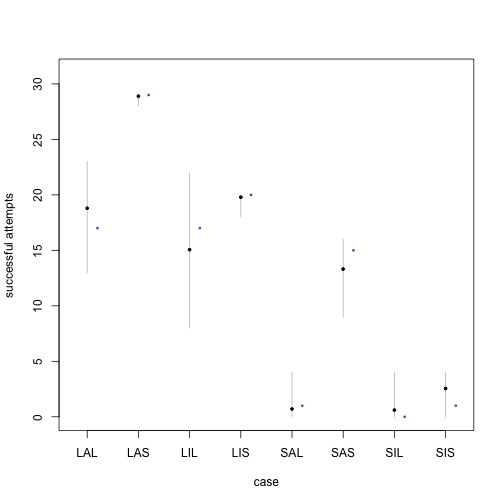
\includegraphics{pirate-plot-b11} \begin{flushleft}
\ttfamily\noindent
\hspace*{\fill}\\
\hlstd{}\hlfunctioncall{plot}\hlkeyword{(}\hlkeyword{(}\hlnumber{1}\hlkeyword{:}\hlnumber{8}\hlkeyword{)}{\ }\hlkeyword{+}{\ }\hlnumber{0.2}\hlkeyword{,}{\ }\hlsymbol{d}\hlkeyword{\usebox{\hlnormalsizeboxdollar}}\hlsymbol{y}\hlkeyword{/}\hlsymbol{d}\hlkeyword{\usebox{\hlnormalsizeboxdollar}}\hlsymbol{n}\hlkeyword{,}{\ }\hlargument{col}{\ }\hlargument{=}{\ }\hlstring{"slateblue"}\hlkeyword{,}{\ }\hlargument{ylab}{\ }\hlargument{=}{\ }\hlstring{"proportion{\ }successful"}\hlkeyword{,}\hspace*{\fill}\\
\hlstd{}{\ }{\ }{\ }{\ }\hlargument{xlab}{\ }\hlargument{=}{\ }\hlstring{"case"}\hlkeyword{,}{\ }\hlargument{xaxt}{\ }\hlargument{=}{\ }\hlstring{"n"}\hlkeyword{,}{\ }\hlargument{xlim}{\ }\hlargument{=}{\ }\hlfunctioncall{c}\hlkeyword{(}\hlnumber{0.75}\hlkeyword{,}{\ }\hlnumber{8.25}\hlkeyword{)}\hlkeyword{,}{\ }\hlargument{pch}{\ }\hlargument{=}{\ }\hlnumber{16}\hlkeyword{,}{\ }\hlargument{ylim}{\ }\hlargument{=}{\ }\hlfunctioncall{c}\hlkeyword{(}\hlnumber{0}\hlkeyword{,}\hspace*{\fill}\\
\hlstd{}{\ }{\ }{\ }{\ }{\ }{\ }{\ }{\ }\hlnumber{1}\hlkeyword{)}\hlkeyword{,}{\ }\hlargument{cex}{\ }\hlargument{=}{\ }\hlnumber{0.5}\hlkeyword{)}\hspace*{\fill}\\
\hlstd{}\hlfunctioncall{axis}\hlkeyword{(}\hlnumber{1}\hlkeyword{,}{\ }\hlargument{at}{\ }\hlargument{=}{\ }\hlnumber{1}\hlkeyword{:}\hlnumber{8}\hlkeyword{,}{\ }\hlargument{labels}{\ }\hlargument{=}{\ }\hlfunctioncall{c}\hlkeyword{(}\hlstring{"LAL"}\hlkeyword{,}{\ }\hlstring{"LAS"}\hlkeyword{,}{\ }\hlstring{"LIL"}\hlkeyword{,}{\ }\hlstring{"LIS"}\hlkeyword{,}\hspace*{\fill}\\
\hlstd{}{\ }{\ }{\ }{\ }\hlstring{"SAL"}\hlkeyword{,}{\ }\hlstring{"SAS"}\hlkeyword{,}{\ }\hlstring{"SIL"}\hlkeyword{,}{\ }\hlstring{"SIS"}\hlkeyword{)}\hlkeyword{)}\hspace*{\fill}\\
\hlstd{}\hlkeyword{for}{\ }\hlkeyword{(}\hlsymbol{i}{\ }\hlkeyword{in}{\ }\hlnumber{1}\hlkeyword{:}\hlnumber{8}\hlkeyword{)}{\ }\hlfunctioncall{lines}\hlkeyword{(}\hlfunctioncall{c}\hlkeyword{(}\hlsymbol{i}\hlkeyword{,}{\ }\hlsymbol{i}\hlkeyword{)}\hlkeyword{,}{\ }\hlfunctioncall{c}\hlkeyword{(}\hlsymbol{y.pred.ci}\hlkeyword{[}\hlkeyword{,}{\ }\hlsymbol{i}\hlkeyword{]}\hlkeyword{/}\hlsymbol{d}\hlkeyword{\usebox{\hlnormalsizeboxdollar}}\hlsymbol{n}\hlkeyword{[}\hlsymbol{i}\hlkeyword{]}\hlkeyword{)}\hlkeyword{,}{\ }\hlargument{col}{\ }\hlargument{=}{\ }\hlstring{"grey"}\hlkeyword{)}\hspace*{\fill}\\
\hlstd{}\hlfunctioncall{points}\hlkeyword{(}\hlnumber{1}\hlkeyword{:}\hlnumber{8}\hlkeyword{,}{\ }\hlsymbol{y.pred}\hlkeyword{/}\hlsymbol{d}\hlkeyword{\usebox{\hlnormalsizeboxdollar}}\hlsymbol{n}\hlkeyword{,}{\ }\hlargument{pch}{\ }\hlargument{=}{\ }\hlnumber{19}\hlkeyword{,}{\ }\hlargument{cex}{\ }\hlargument{=}{\ }\hlnumber{0.5}\hlkeyword{,}{\ }\hlargument{col}{\ }\hlargument{=}{\ }\hlstring{"black"}\hlkeyword{)}\mbox{}
\normalfont
\end{flushleft}
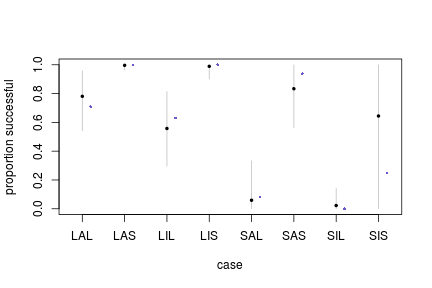
\includegraphics{pirate-plot-b12} \begin{flushleft}
\ttfamily\noindent
\hspace*{\fill}\\
\hlstd{}\hlcomment{\usebox{\hlnormalsizeboxhash}par(op)}\mbox{}
\normalfont
\end{flushleft}
\end{kframe}}
\end{knitrout}


Counts of success plot (first figure):

shows heterogeneity in relative frequency of successful attempts across encounter types

confidence intervals and point estimates easier to interpret relative to the data

Proportional plot (second figure): 

shows heterogeneity in probability across encounter types

confidence intervals provide better depiction of uncertainty in outcome



\subsubsection*{(C)}

We'd like to improve the model, so we  fit the interaction model 
\begin{align*}
&y_i \sim {\rm Binomial} ( p_i , n_i)\\
&\log \frac{p_i}{1-p_i} = \alpha + \beta_P P_i + \beta_V V_i + \beta_A A_i + \beta_{PA} P_i \cdot A_i
\end{align*}

\begin{knitrout}
\definecolor{shadecolor}{rgb}{.97, .97, .97}{\color{fgcolor}\begin{kframe}
\begin{flushleft}
\ttfamily\noindent
\hlsymbol{m1c}{\ }\hlassignement{\usebox{\hlnormalsizeboxlessthan}-}{\ }\hlfunctioncall{mle2}\hlkeyword{(}\hlsymbol{y}{\ }\hlkeyword{\urltilda{}}{\ }\hlfunctioncall{dbinom}\hlkeyword{(}\hlargument{prob}{\ }\hlargument{=}{\ }\hlfunctioncall{logistic}\hlkeyword{(}\hlsymbol{a}{\ }\hlkeyword{+}{\ }\hlsymbol{bP}{\ }\hlkeyword{*}{\ }\hlsymbol{pirateL}{\ }\hlkeyword{+}\hspace*{\fill}\\
\hlstd{}{\ }{\ }{\ }{\ }\hlsymbol{bV}{\ }\hlkeyword{*}{\ }\hlsymbol{victimL}{\ }\hlkeyword{+}{\ }\hlsymbol{bA}{\ }\hlkeyword{*}{\ }\hlsymbol{pirateA}{\ }\hlkeyword{+}{\ }\hlsymbol{bPA}{\ }\hlkeyword{*}{\ }\hlsymbol{pirateL}{\ }\hlkeyword{*}{\ }\hlsymbol{pirateA}\hlkeyword{)}\hlkeyword{,}{\ }\hlargument{size}{\ }\hlargument{=}{\ }\hlsymbol{n}\hlkeyword{)}\hlkeyword{,}\hspace*{\fill}\\
\hlstd{}{\ }{\ }{\ }{\ }\hlargument{data}{\ }\hlargument{=}{\ }\hlsymbol{d}\hlkeyword{,}{\ }\hlargument{start}{\ }\hlargument{=}{\ }\hlfunctioncall{list}\hlkeyword{(}\hlargument{a}{\ }\hlargument{=}{\ }\hlfunctioncall{mean}\hlkeyword{(}\hlsymbol{d}\hlkeyword{\usebox{\hlnormalsizeboxdollar}}\hlsymbol{y}\hlkeyword{)}\hlkeyword{,}{\ }\hlargument{bP}{\ }\hlargument{=}{\ }\hlnumber{0}\hlkeyword{,}{\ }\hlargument{bV}{\ }\hlargument{=}{\ }\hlnumber{0}\hlkeyword{,}{\ }\hlargument{bA}{\ }\hlargument{=}{\ }\hlnumber{0}\hlkeyword{,}{\ }\hlargument{bPA}{\ }\hlargument{=}{\ }\hlnumber{0}\hlkeyword{)}\hlkeyword{)}\hspace*{\fill}\\
\hlstd{}\hlsymbol{p.m1c}{\ }\hlassignement{\usebox{\hlnormalsizeboxlessthan}-}{\ }\hlfunctioncall{precis}\hlkeyword{(}\hlsymbol{m1c}\hlkeyword{)}\hspace*{\fill}\\
\hlstd{}\hspace*{\fill}\\
\hlstd{}\hlfunctioncall{compare}\hlkeyword{(}\hlsymbol{m1a}\hlkeyword{,}{\ }\hlsymbol{m1c}\hlkeyword{,}{\ }\hlargument{nobs}{\ }\hlargument{=}{\ }\hlfunctioncall{sum}\hlkeyword{(}\hlsymbol{d}\hlkeyword{\usebox{\hlnormalsizeboxdollar}}\hlsymbol{n}\hlkeyword{)}\hlkeyword{)}\mbox{}
\normalfont
\end{flushleft}
\begin{verbatim}
##     k  AICc   BIC w.AICc   w.BIC dAICc  dBIC
## m1c 5 23.46 23.47 0.9043 0.90653 0.000 0.000
## m1a 4 27.95 28.01 0.0957 0.09347 4.492 4.544
\end{verbatim}
\end{kframe}}
\end{knitrout}



\begin{knitrout}
\definecolor{shadecolor}{rgb}{.97, .97, .97}{\color{fgcolor}\begin{kframe}
\begin{flushleft}
\ttfamily\noindent
\hlfunctioncall{rm}\hlkeyword{(}\hlargument{list}{\ }\hlargument{=}{\ }\hlfunctioncall{c}\hlkeyword{(}\hlstring{"post"}\hlkeyword{,}{\ }\hlstring{"y.pred"}\hlkeyword{,}{\ }\hlstring{"y.pred.ci"}\hlkeyword{)}\hlkeyword{)}\mbox{}
\normalfont
\end{flushleft}
\begin{verbatim}
## Warning message: object 'post' not found
\end{verbatim}
\begin{verbatim}
## Warning message: object 'y.pred' not found
\end{verbatim}
\begin{verbatim}
## Warning message: object 'y.pred.ci' not found
\end{verbatim}
\begin{flushleft}
\ttfamily\noindent
\hlsymbol{post}{\ }\hlassignement{\usebox{\hlnormalsizeboxlessthan}-}{\ }\hlfunctioncall{sample.naive.posterior}\hlkeyword{(}\hlfunctioncall{list}\hlkeyword{(}\hlsymbol{m1a}\hlkeyword{,}{\ }\hlsymbol{m1c}\hlkeyword{)}\hlkeyword{,}{\ }\hlargument{method}{\ }\hlargument{=}{\ }\hlstring{"AICc"}\hlkeyword{,}\hspace*{\fill}\\
\hlstd{}{\ }{\ }{\ }{\ }\hlargument{nobs}{\ }\hlargument{=}{\ }\hlfunctioncall{sum}\hlkeyword{(}\hlsymbol{d}\hlkeyword{\usebox{\hlnormalsizeboxdollar}}\hlsymbol{n}\hlkeyword{)}\hlkeyword{,}{\ }\hlargument{n}{\ }\hlargument{=}{\ }\hlnumber{30000}\hlkeyword{)}\hspace*{\fill}\\
\hlstd{}\hspace*{\fill}\\
\hlstd{}\hlsymbol{y.pred}{\ }\hlassignement{\usebox{\hlnormalsizeboxlessthan}-}{\ }\hlfunctioncall{sapply}\hlkeyword{(}\hlnumber{1}\hlkeyword{:}\hlfunctioncall{nrow}\hlkeyword{(}\hlsymbol{d}\hlkeyword{)}\hlkeyword{,}{\ }\hlkeyword{function}\hlkeyword{(}\hlformalargs{i}\hlkeyword{)}{\ }\hlfunctioncall{mean}\hlkeyword{(}\hlfunctioncall{rbinom}\hlkeyword{(}\hlargument{n}{\ }\hlargument{=}{\ }\hlnumber{10000}\hlkeyword{,}\hspace*{\fill}\\
\hlstd{}{\ }{\ }{\ }{\ }\hlargument{prob}{\ }\hlargument{=}{\ }\hlfunctioncall{logistic}\hlkeyword{(}\hlsymbol{post}\hlkeyword{\usebox{\hlnormalsizeboxdollar}}\hlsymbol{a}{\ }\hlkeyword{+}{\ }\hlsymbol{post}\hlkeyword{\usebox{\hlnormalsizeboxdollar}}\hlsymbol{bP}{\ }\hlkeyword{*}{\ }\hlsymbol{d}\hlkeyword{\usebox{\hlnormalsizeboxdollar}}\hlsymbol{pirateL}\hlkeyword{[}\hlsymbol{i}\hlkeyword{]}{\ }\hlkeyword{+}{\ }\hlsymbol{post}\hlkeyword{\usebox{\hlnormalsizeboxdollar}}\hlsymbol{bV}{\ }\hlkeyword{*}{\ }\hlsymbol{d}\hlkeyword{\usebox{\hlnormalsizeboxdollar}}\hlsymbol{victimL}\hlkeyword{[}\hlsymbol{i}\hlkeyword{]}{\ }\hlkeyword{+}\hspace*{\fill}\\
\hlstd{}{\ }{\ }{\ }{\ }{\ }{\ }{\ }{\ }\hlsymbol{post}\hlkeyword{\usebox{\hlnormalsizeboxdollar}}\hlsymbol{bA}{\ }\hlkeyword{*}{\ }\hlsymbol{d}\hlkeyword{\usebox{\hlnormalsizeboxdollar}}\hlsymbol{pirateA}\hlkeyword{[}\hlsymbol{i}\hlkeyword{]}{\ }\hlkeyword{+}{\ }\hlsymbol{post}\hlkeyword{\usebox{\hlnormalsizeboxdollar}}\hlsymbol{bPA}{\ }\hlkeyword{*}{\ }\hlsymbol{d}\hlkeyword{\usebox{\hlnormalsizeboxdollar}}\hlsymbol{pirateL}\hlkeyword{[}\hlsymbol{i}\hlkeyword{]}{\ }\hlkeyword{*}{\ }\hlsymbol{d}\hlkeyword{\usebox{\hlnormalsizeboxdollar}}\hlsymbol{pirateA}\hlkeyword{[}\hlsymbol{i}\hlkeyword{]}\hlkeyword{)}\hlkeyword{,}\hspace*{\fill}\\
\hlstd{}{\ }{\ }{\ }{\ }\hlargument{size}{\ }\hlargument{=}{\ }\hlsymbol{d}\hlkeyword{\usebox{\hlnormalsizeboxdollar}}\hlsymbol{n}\hlkeyword{[}\hlsymbol{i}\hlkeyword{]}\hlkeyword{)}\hlkeyword{)}\hlkeyword{)}\hspace*{\fill}\\
\hlstd{}\hspace*{\fill}\\
\hlstd{}\hlsymbol{y.pred.ci}{\ }\hlassignement{\usebox{\hlnormalsizeboxlessthan}-}{\ }\hlfunctioncall{sapply}\hlkeyword{(}\hlnumber{1}\hlkeyword{:}\hlfunctioncall{nrow}\hlkeyword{(}\hlsymbol{d}\hlkeyword{)}\hlkeyword{,}{\ }\hlkeyword{function}\hlkeyword{(}\hlformalargs{i}\hlkeyword{)}{\ }\hlfunctioncall{PCI}\hlkeyword{(}\hlfunctioncall{rbinom}\hlkeyword{(}\hlargument{n}{\ }\hlargument{=}{\ }\hlnumber{10000}\hlkeyword{,}\hspace*{\fill}\\
\hlstd{}{\ }{\ }{\ }{\ }\hlargument{prob}{\ }\hlargument{=}{\ }\hlfunctioncall{logistic}\hlkeyword{(}\hlsymbol{post}\hlkeyword{\usebox{\hlnormalsizeboxdollar}}\hlsymbol{a}{\ }\hlkeyword{+}{\ }\hlsymbol{post}\hlkeyword{\usebox{\hlnormalsizeboxdollar}}\hlsymbol{bP}{\ }\hlkeyword{*}{\ }\hlsymbol{d}\hlkeyword{\usebox{\hlnormalsizeboxdollar}}\hlsymbol{pirateL}\hlkeyword{[}\hlsymbol{i}\hlkeyword{]}{\ }\hlkeyword{+}{\ }\hlsymbol{post}\hlkeyword{\usebox{\hlnormalsizeboxdollar}}\hlsymbol{bV}{\ }\hlkeyword{*}{\ }\hlsymbol{d}\hlkeyword{\usebox{\hlnormalsizeboxdollar}}\hlsymbol{victimL}\hlkeyword{[}\hlsymbol{i}\hlkeyword{]}{\ }\hlkeyword{+}\hspace*{\fill}\\
\hlstd{}{\ }{\ }{\ }{\ }{\ }{\ }{\ }{\ }\hlsymbol{post}\hlkeyword{\usebox{\hlnormalsizeboxdollar}}\hlsymbol{bA}{\ }\hlkeyword{*}{\ }\hlsymbol{d}\hlkeyword{\usebox{\hlnormalsizeboxdollar}}\hlsymbol{pirateA}\hlkeyword{[}\hlsymbol{i}\hlkeyword{]}{\ }\hlkeyword{+}{\ }\hlsymbol{post}\hlkeyword{\usebox{\hlnormalsizeboxdollar}}\hlsymbol{bPA}{\ }\hlkeyword{*}{\ }\hlsymbol{d}\hlkeyword{\usebox{\hlnormalsizeboxdollar}}\hlsymbol{pirateL}\hlkeyword{[}\hlsymbol{i}\hlkeyword{]}{\ }\hlkeyword{*}{\ }\hlsymbol{d}\hlkeyword{\usebox{\hlnormalsizeboxdollar}}\hlsymbol{pirateA}\hlkeyword{[}\hlsymbol{i}\hlkeyword{]}\hlkeyword{)}\hlkeyword{,}\hspace*{\fill}\\
\hlstd{}{\ }{\ }{\ }{\ }\hlargument{size}{\ }\hlargument{=}{\ }\hlsymbol{d}\hlkeyword{\usebox{\hlnormalsizeboxdollar}}\hlsymbol{n}\hlkeyword{[}\hlsymbol{i}\hlkeyword{]}\hlkeyword{)}\hlkeyword{)}\hlkeyword{)}\hspace*{\fill}\\
\hlstd{}\hspace*{\fill}\\
\hlstd{}\hlcomment{\usebox{\hlnormalsizeboxhash}op{\ }\usebox{\hlnormalsizeboxlessthan}-{\ }par(mfrow=c(2,1))}\hspace*{\fill}\\
\hlstd{}\hlfunctioncall{plot}\hlkeyword{(}\hlkeyword{(}\hlnumber{1}\hlkeyword{:}\hlnumber{8}\hlkeyword{)}{\ }\hlkeyword{+}{\ }\hlnumber{0.2}\hlkeyword{,}{\ }\hlsymbol{d}\hlkeyword{\usebox{\hlnormalsizeboxdollar}}\hlsymbol{y}\hlkeyword{,}{\ }\hlargument{col}{\ }\hlargument{=}{\ }\hlstring{"slateblue"}\hlkeyword{,}{\ }\hlargument{ylab}{\ }\hlargument{=}{\ }\hlstring{"successful{\ }attempts"}\hlkeyword{,}\hspace*{\fill}\\
\hlstd{}{\ }{\ }{\ }{\ }\hlargument{xlab}{\ }\hlargument{=}{\ }\hlstring{"case"}\hlkeyword{,}{\ }\hlargument{xaxt}{\ }\hlargument{=}{\ }\hlstring{"n"}\hlkeyword{,}{\ }\hlargument{xlim}{\ }\hlargument{=}{\ }\hlfunctioncall{c}\hlkeyword{(}\hlnumber{0.75}\hlkeyword{,}{\ }\hlnumber{8.25}\hlkeyword{)}\hlkeyword{,}{\ }\hlargument{pch}{\ }\hlargument{=}{\ }\hlnumber{16}\hlkeyword{,}{\ }\hlargument{ylim}{\ }\hlargument{=}{\ }\hlfunctioncall{c}\hlkeyword{(}\hlnumber{0}\hlkeyword{,}\hspace*{\fill}\\
\hlstd{}{\ }{\ }{\ }{\ }{\ }{\ }{\ }{\ }\hlnumber{31}\hlkeyword{)}\hlkeyword{,}{\ }\hlargument{cex}{\ }\hlargument{=}{\ }\hlnumber{0.5}\hlkeyword{)}\hspace*{\fill}\\
\hlstd{}\hlfunctioncall{axis}\hlkeyword{(}\hlnumber{1}\hlkeyword{,}{\ }\hlargument{at}{\ }\hlargument{=}{\ }\hlnumber{1}\hlkeyword{:}\hlnumber{8}\hlkeyword{,}{\ }\hlargument{labels}{\ }\hlargument{=}{\ }\hlfunctioncall{c}\hlkeyword{(}\hlstring{"LAL"}\hlkeyword{,}{\ }\hlstring{"LAS"}\hlkeyword{,}{\ }\hlstring{"LIL"}\hlkeyword{,}{\ }\hlstring{"LIS"}\hlkeyword{,}\hspace*{\fill}\\
\hlstd{}{\ }{\ }{\ }{\ }\hlstring{"SAL"}\hlkeyword{,}{\ }\hlstring{"SAS"}\hlkeyword{,}{\ }\hlstring{"SIL"}\hlkeyword{,}{\ }\hlstring{"SIS"}\hlkeyword{)}\hlkeyword{)}\hspace*{\fill}\\
\hlstd{}\hlkeyword{for}{\ }\hlkeyword{(}\hlsymbol{i}{\ }\hlkeyword{in}{\ }\hlnumber{1}\hlkeyword{:}\hlnumber{8}\hlkeyword{)}{\ }\hlfunctioncall{lines}\hlkeyword{(}\hlfunctioncall{c}\hlkeyword{(}\hlsymbol{i}\hlkeyword{,}{\ }\hlsymbol{i}\hlkeyword{)}\hlkeyword{,}{\ }\hlfunctioncall{c}\hlkeyword{(}\hlsymbol{y.pred.ci}\hlkeyword{[}\hlkeyword{,}{\ }\hlsymbol{i}\hlkeyword{]}\hlkeyword{)}\hlkeyword{,}{\ }\hlargument{col}{\ }\hlargument{=}{\ }\hlstring{"grey"}\hlkeyword{)}\hspace*{\fill}\\
\hlstd{}\hlfunctioncall{points}\hlkeyword{(}\hlnumber{1}\hlkeyword{:}\hlnumber{8}\hlkeyword{,}{\ }\hlsymbol{y.pred}\hlkeyword{,}{\ }\hlargument{pch}{\ }\hlargument{=}{\ }\hlnumber{19}\hlkeyword{,}{\ }\hlargument{cex}{\ }\hlargument{=}{\ }\hlnumber{0.5}\hlkeyword{,}{\ }\hlargument{col}{\ }\hlargument{=}{\ }\hlstring{"black"}\hlkeyword{)}\mbox{}
\normalfont
\end{flushleft}
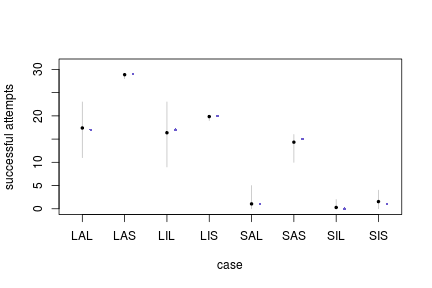
\includegraphics{better-model-fig1} \begin{flushleft}
\ttfamily\noindent
\hspace*{\fill}\\
\hlstd{}\hlfunctioncall{plot}\hlkeyword{(}\hlkeyword{(}\hlnumber{1}\hlkeyword{:}\hlnumber{8}\hlkeyword{)}{\ }\hlkeyword{+}{\ }\hlnumber{0.2}\hlkeyword{,}{\ }\hlsymbol{d}\hlkeyword{\usebox{\hlnormalsizeboxdollar}}\hlsymbol{y}\hlkeyword{/}\hlsymbol{d}\hlkeyword{\usebox{\hlnormalsizeboxdollar}}\hlsymbol{n}\hlkeyword{,}{\ }\hlargument{col}{\ }\hlargument{=}{\ }\hlstring{"slateblue"}\hlkeyword{,}{\ }\hlargument{ylab}{\ }\hlargument{=}{\ }\hlstring{"proportion{\ }successful"}\hlkeyword{,}\hspace*{\fill}\\
\hlstd{}{\ }{\ }{\ }{\ }\hlargument{xlab}{\ }\hlargument{=}{\ }\hlstring{"case"}\hlkeyword{,}{\ }\hlargument{xaxt}{\ }\hlargument{=}{\ }\hlstring{"n"}\hlkeyword{,}{\ }\hlargument{xlim}{\ }\hlargument{=}{\ }\hlfunctioncall{c}\hlkeyword{(}\hlnumber{0.75}\hlkeyword{,}{\ }\hlnumber{8.25}\hlkeyword{)}\hlkeyword{,}{\ }\hlargument{pch}{\ }\hlargument{=}{\ }\hlnumber{16}\hlkeyword{,}{\ }\hlargument{ylim}{\ }\hlargument{=}{\ }\hlfunctioncall{c}\hlkeyword{(}\hlnumber{0}\hlkeyword{,}\hspace*{\fill}\\
\hlstd{}{\ }{\ }{\ }{\ }{\ }{\ }{\ }{\ }\hlnumber{1}\hlkeyword{)}\hlkeyword{,}{\ }\hlargument{cex}{\ }\hlargument{=}{\ }\hlnumber{0.5}\hlkeyword{)}\hspace*{\fill}\\
\hlstd{}\hlfunctioncall{axis}\hlkeyword{(}\hlnumber{1}\hlkeyword{,}{\ }\hlargument{at}{\ }\hlargument{=}{\ }\hlnumber{1}\hlkeyword{:}\hlnumber{8}\hlkeyword{,}{\ }\hlargument{labels}{\ }\hlargument{=}{\ }\hlfunctioncall{c}\hlkeyword{(}\hlstring{"LAL"}\hlkeyword{,}{\ }\hlstring{"LAS"}\hlkeyword{,}{\ }\hlstring{"LIL"}\hlkeyword{,}{\ }\hlstring{"LIS"}\hlkeyword{,}\hspace*{\fill}\\
\hlstd{}{\ }{\ }{\ }{\ }\hlstring{"SAL"}\hlkeyword{,}{\ }\hlstring{"SAS"}\hlkeyword{,}{\ }\hlstring{"SIL"}\hlkeyword{,}{\ }\hlstring{"SIS"}\hlkeyword{)}\hlkeyword{)}\hspace*{\fill}\\
\hlstd{}\hlkeyword{for}{\ }\hlkeyword{(}\hlsymbol{i}{\ }\hlkeyword{in}{\ }\hlnumber{1}\hlkeyword{:}\hlnumber{8}\hlkeyword{)}{\ }\hlfunctioncall{lines}\hlkeyword{(}\hlfunctioncall{c}\hlkeyword{(}\hlsymbol{i}\hlkeyword{,}{\ }\hlsymbol{i}\hlkeyword{)}\hlkeyword{,}{\ }\hlfunctioncall{c}\hlkeyword{(}\hlsymbol{y.pred.ci}\hlkeyword{[}\hlkeyword{,}{\ }\hlsymbol{i}\hlkeyword{]}\hlkeyword{/}\hlsymbol{d}\hlkeyword{\usebox{\hlnormalsizeboxdollar}}\hlsymbol{n}\hlkeyword{[}\hlsymbol{i}\hlkeyword{]}\hlkeyword{)}\hlkeyword{,}{\ }\hlargument{col}{\ }\hlargument{=}{\ }\hlstring{"grey"}\hlkeyword{)}\hspace*{\fill}\\
\hlstd{}\hlfunctioncall{points}\hlkeyword{(}\hlnumber{1}\hlkeyword{:}\hlnumber{8}\hlkeyword{,}{\ }\hlsymbol{y.pred}\hlkeyword{/}\hlsymbol{d}\hlkeyword{\usebox{\hlnormalsizeboxdollar}}\hlsymbol{n}\hlkeyword{,}{\ }\hlargument{pch}{\ }\hlargument{=}{\ }\hlnumber{19}\hlkeyword{,}{\ }\hlargument{cex}{\ }\hlargument{=}{\ }\hlnumber{0.5}\hlkeyword{,}{\ }\hlargument{col}{\ }\hlargument{=}{\ }\hlstring{"black"}\hlkeyword{)}\mbox{}
\normalfont
\end{flushleft}
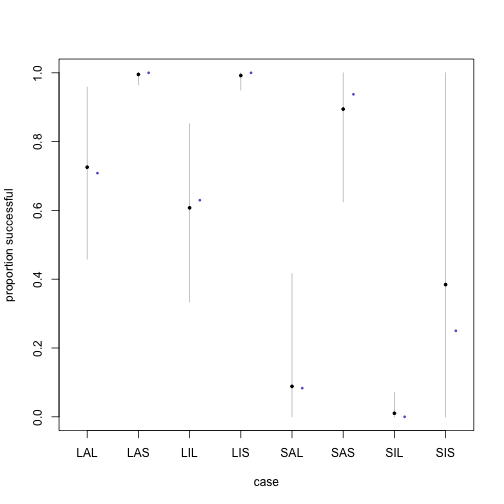
\includegraphics{better-model-fig2} \begin{flushleft}
\ttfamily\noindent
\hspace*{\fill}\\
\hlstd{}\hlcomment{\usebox{\hlnormalsizeboxhash}par(op)}\mbox{}
\normalfont
\end{flushleft}
\end{kframe}}
\end{knitrout}


\subsection*{Herptiles}

\begin{knitrout}
\definecolor{shadecolor}{rgb}{.97, .97, .97}{\color{fgcolor}\begin{kframe}
\begin{flushleft}
\ttfamily\noindent
\hlfunctioncall{data}\hlkeyword{(}\hlsymbol{salamanders}\hlkeyword{)}\hspace*{\fill}\\
\hlstd{}\hlsymbol{d}{\ }\hlassignement{\usebox{\hlnormalsizeboxlessthan}-}{\ }\hlsymbol{salamanders}\hspace*{\fill}\\
\hlstd{}\hlfunctioncall{head}\hlkeyword{(}\hlsymbol{d}\hlkeyword{,}{\ }\hlargument{n}{\ }\hlargument{=}{\ }\hlnumber{1}\hlkeyword{)}\mbox{}
\normalfont
\end{flushleft}
\begin{verbatim}
##   SITE SALAMAN PCTCOVER FORESTAGE
## 1    1      13       85       316
\end{verbatim}
\begin{flushleft}
\ttfamily\noindent
\hlsymbol{d}\hlkeyword{\usebox{\hlnormalsizeboxdollar}}\hlsymbol{pc}{\ }\hlassignement{\usebox{\hlnormalsizeboxlessthan}-}{\ }\hlsymbol{d}\hlkeyword{\usebox{\hlnormalsizeboxdollar}}\hlsymbol{PCTCOVER}{\ }\hlkeyword{-}{\ }\hlfunctioncall{mean}\hlkeyword{(}\hlsymbol{d}\hlkeyword{\usebox{\hlnormalsizeboxdollar}}\hlsymbol{PCTCOVER}\hlkeyword{)}\hspace*{\fill}\\
\hlstd{}\hlsymbol{d}\hlkeyword{\usebox{\hlnormalsizeboxdollar}}\hlsymbol{fs}{\ }\hlassignement{\usebox{\hlnormalsizeboxlessthan}-}{\ }\hlsymbol{d}\hlkeyword{\usebox{\hlnormalsizeboxdollar}}\hlsymbol{FORESTAGE}{\ }\hlkeyword{-}{\ }\hlfunctioncall{mean}\hlkeyword{(}\hlsymbol{d}\hlkeyword{\usebox{\hlnormalsizeboxdollar}}\hlsymbol{FORESTAGE}\hlkeyword{)}\mbox{}
\normalfont
\end{flushleft}
\end{kframe}}
\end{knitrout}


The data set includes counts of salamanders in each plot (SALAMAN), as well as percent (PCTCOVER) and age (FORESTAGE) of ground cover.
I recenter the predictors. 


\subsubsection*{(A)}

I model the count variable SALAMAN as a Poisson variable:
\begin{align*}
&S_i \sim {\rm Poisson} ( \lambda_i)\\
&\log \lambda = \alpha + \beta_P *P_i
\end{align*}
where $S_i$ is SALAMAN and $P_i$ is PCTCOVER

\begin{knitrout}
\definecolor{shadecolor}{rgb}{.97, .97, .97}{\color{fgcolor}\begin{kframe}
\begin{flushleft}
\ttfamily\noindent
\hlsymbol{m2a}{\ }\hlassignement{\usebox{\hlnormalsizeboxlessthan}-}{\ }\hlfunctioncall{mle2}\hlkeyword{(}\hlsymbol{SALAMAN}{\ }\hlkeyword{\urltilda{}}{\ }\hlfunctioncall{dpois}\hlkeyword{(}\hlargument{lambda}{\ }\hlargument{=}{\ }\hlfunctioncall{exp}\hlkeyword{(}\hlsymbol{a}{\ }\hlkeyword{+}{\ }\hlsymbol{b.P}{\ }\hlkeyword{*}{\ }\hlsymbol{pc}\hlkeyword{)}\hlkeyword{)}\hlkeyword{,}\hspace*{\fill}\\
\hlstd{}{\ }{\ }{\ }{\ }\hlargument{data}{\ }\hlargument{=}{\ }\hlsymbol{d}\hlkeyword{,}{\ }\hlargument{start}{\ }\hlargument{=}{\ }\hlfunctioncall{list}\hlkeyword{(}\hlargument{a}{\ }\hlargument{=}{\ }\hlfunctioncall{log}\hlkeyword{(}\hlfunctioncall{mean}\hlkeyword{(}\hlsymbol{d}\hlkeyword{\usebox{\hlnormalsizeboxdollar}}\hlsymbol{SALAMAN}\hlkeyword{)}\hlkeyword{)}\hlkeyword{,}{\ }\hlargument{b.P}{\ }\hlargument{=}{\ }\hlnumber{0}\hlkeyword{)}\hlkeyword{)}\hspace*{\fill}\\
\hlstd{}\hlfunctioncall{precis}\hlkeyword{(}\hlsymbol{m2a}\hlkeyword{)}\mbox{}
\normalfont
\end{flushleft}
\begin{verbatim}
##     Estimate Std. Error   2.5%  97.5%
## a     0.4262   0.158826 0.1149 0.7375
## b.P   0.0325   0.005409 0.0219 0.0431
\end{verbatim}
\end{kframe}}
\end{knitrout}



\begin{knitrout}
\definecolor{shadecolor}{rgb}{.97, .97, .97}{\color{fgcolor}\begin{kframe}
\begin{flushleft}
\ttfamily\noindent
\hlsymbol{post}{\ }\hlassignement{\usebox{\hlnormalsizeboxlessthan}-}{\ }\hlfunctioncall{sample.naive.posterior}\hlkeyword{(}\hlsymbol{m2a}\hlkeyword{)}\hspace*{\fill}\\
\hlstd{}\hlsymbol{pct.seq}{\ }\hlassignement{\usebox{\hlnormalsizeboxlessthan}-}{\ }\hlfunctioncall{seq}\hlkeyword{(}\hlfunctioncall{min}\hlkeyword{(}\hlsymbol{d}\hlkeyword{\usebox{\hlnormalsizeboxdollar}}\hlsymbol{pc}\hlkeyword{)}\hlkeyword{,}{\ }\hlfunctioncall{max}\hlkeyword{(}\hlsymbol{d}\hlkeyword{\usebox{\hlnormalsizeboxdollar}}\hlsymbol{pc}\hlkeyword{)}\hlkeyword{,}{\ }\hlargument{length.out}{\ }\hlargument{=}{\ }\hlnumber{100}\hlkeyword{)}\hspace*{\fill}\\
\hlstd{}\hspace*{\fill}\\
\hlstd{}\hlsymbol{y.pred}{\ }\hlassignement{\usebox{\hlnormalsizeboxlessthan}-}{\ }\hlfunctioncall{sapply}\hlkeyword{(}\hlsymbol{pct.seq}\hlkeyword{,}{\ }\hlkeyword{function}\hlkeyword{(}\hlformalargs{z}\hlkeyword{)}{\ }\hlfunctioncall{mean}\hlkeyword{(}\hlfunctioncall{exp}\hlkeyword{(}\hlsymbol{post}\hlkeyword{\usebox{\hlnormalsizeboxdollar}}\hlsymbol{a}{\ }\hlkeyword{+}{\ }\hlsymbol{post}\hlkeyword{\usebox{\hlnormalsizeboxdollar}}\hlsymbol{b.P}{\ }\hlkeyword{*}\hspace*{\fill}\\
\hlstd{}{\ }{\ }{\ }{\ }\hlsymbol{z}\hlkeyword{)}\hlkeyword{)}\hlkeyword{)}\hspace*{\fill}\\
\hlstd{}\hlsymbol{n}\mbox{}
\normalfont
\end{flushleft}
\begin{verbatim}
## Error: object 'n' not found
\end{verbatim}
\begin{flushleft}
\ttfamily\noindent
\hlsymbol{y.pred.ci}{\ }\hlassignement{\usebox{\hlnormalsizeboxlessthan}-}{\ }\hlfunctioncall{sapply}\hlkeyword{(}\hlsymbol{pct.seq}\hlkeyword{,}{\ }\hlkeyword{function}\hlkeyword{(}\hlformalargs{z}\hlkeyword{)}{\ }\hlfunctioncall{PCI}\hlkeyword{(}\hlfunctioncall{exp}\hlkeyword{(}\hlsymbol{post}\hlkeyword{\usebox{\hlnormalsizeboxdollar}}\hlsymbol{a}{\ }\hlkeyword{+}\hspace*{\fill}\\
\hlstd{}{\ }{\ }{\ }{\ }\hlsymbol{post}\hlkeyword{\usebox{\hlnormalsizeboxdollar}}\hlsymbol{b.P}{\ }\hlkeyword{*}{\ }\hlsymbol{z}\hlkeyword{)}\hlkeyword{)}\hlkeyword{)}\hspace*{\fill}\\
\hlstd{}\hspace*{\fill}\\
\hlstd{}\hlsymbol{y.pred.pi}{\ }\hlassignement{\usebox{\hlnormalsizeboxlessthan}-}{\ }\hlfunctioncall{sapply}\hlkeyword{(}\hlsymbol{pct.seq}\hlkeyword{,}{\ }\hlkeyword{function}\hlkeyword{(}\hlformalargs{z}\hlkeyword{)}{\ }\hlfunctioncall{PCI}\hlkeyword{(}\hlfunctioncall{rpois}\hlkeyword{(}\hlargument{n}{\ }\hlargument{=}{\ }\hlnumber{30000}\hlkeyword{,}\hspace*{\fill}\\
\hlstd{}{\ }{\ }{\ }{\ }\hlargument{lambda}{\ }\hlargument{=}{\ }\hlfunctioncall{exp}\hlkeyword{(}\hlsymbol{post}\hlkeyword{\usebox{\hlnormalsizeboxdollar}}\hlsymbol{a}{\ }\hlkeyword{+}{\ }\hlsymbol{post}\hlkeyword{\usebox{\hlnormalsizeboxdollar}}\hlsymbol{b.P}{\ }\hlkeyword{*}{\ }\hlsymbol{z}\hlkeyword{)}\hlkeyword{)}\hlkeyword{)}\hlkeyword{)}\hspace*{\fill}\\
\hlstd{}\hspace*{\fill}\\
\hlstd{}\hspace*{\fill}\\
\hlstd{}\hlfunctioncall{plot}\hlkeyword{(}\hlsymbol{SALAMAN}{\ }\hlkeyword{\urltilda{}}{\ }\hlsymbol{pc}\hlkeyword{,}{\ }\hlargument{data}{\ }\hlargument{=}{\ }\hlsymbol{d}\hlkeyword{,}{\ }\hlargument{col}{\ }\hlargument{=}{\ }\hlfunctioncall{col.alpha}\hlkeyword{(}\hlstring{"gray"}\hlkeyword{,}{\ }\hlnumber{0.9}\hlkeyword{)}\hlkeyword{,}\hspace*{\fill}\\
\hlstd{}{\ }{\ }{\ }{\ }\hlargument{pch}{\ }\hlargument{=}{\ }\hlnumber{19}\hlkeyword{)}\hspace*{\fill}\\
\hlstd{}\hlfunctioncall{lines}\hlkeyword{(}\hlsymbol{pct.seq}\hlkeyword{,}{\ }\hlsymbol{y.pred}\hlkeyword{)}\hspace*{\fill}\\
\hlstd{}\hlfunctioncall{lines}\hlkeyword{(}\hlsymbol{pct.seq}\hlkeyword{,}{\ }\hlsymbol{y.pred.ci}\hlkeyword{[}\hlnumber{1}\hlkeyword{,}{\ }\hlkeyword{]}\hlkeyword{,}{\ }\hlargument{lty}{\ }\hlargument{=}{\ }\hlnumber{2}\hlkeyword{)}\hspace*{\fill}\\
\hlstd{}\hlfunctioncall{lines}\hlkeyword{(}\hlsymbol{pct.seq}\hlkeyword{,}{\ }\hlsymbol{y.pred.ci}\hlkeyword{[}\hlnumber{2}\hlkeyword{,}{\ }\hlkeyword{]}\hlkeyword{,}{\ }\hlargument{lty}{\ }\hlargument{=}{\ }\hlnumber{2}\hlkeyword{)}\hspace*{\fill}\\
\hlstd{}\hlfunctioncall{lines}\hlkeyword{(}\hlsymbol{pct.seq}\hlkeyword{,}{\ }\hlsymbol{y.pred.pi}\hlkeyword{[}\hlnumber{1}\hlkeyword{,}{\ }\hlkeyword{]}\hlkeyword{,}{\ }\hlargument{lty}{\ }\hlargument{=}{\ }\hlnumber{3}\hlkeyword{)}\hspace*{\fill}\\
\hlstd{}\hlfunctioncall{lines}\hlkeyword{(}\hlsymbol{pct.seq}\hlkeyword{,}{\ }\hlsymbol{y.pred.pi}\hlkeyword{[}\hlnumber{2}\hlkeyword{,}{\ }\hlkeyword{]}\hlkeyword{,}{\ }\hlargument{lty}{\ }\hlargument{=}{\ }\hlnumber{3}\hlkeyword{)}\mbox{}
\normalfont
\end{flushleft}
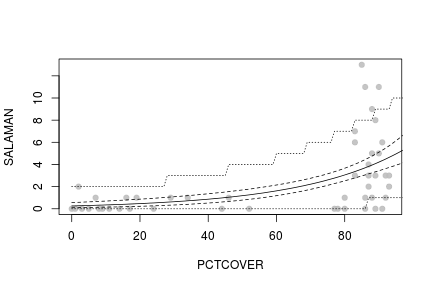
\includegraphics{sal-fig} \begin{flushleft}
\ttfamily\noindent
\hlcomment{\usebox{\hlnormalsizeboxhash}todo{\ }rewrite{\ }x{\ }axis{\ }to{\ }0:100,{\ }see{\ }RM\usebox{\hlnormalsizeboxsinglequote}s{\ }code{\ }above}\mbox{}
\normalfont
\end{flushleft}
\end{kframe}}
\end{knitrout}


The model does a good job at low percent ground cover, with all observation falling within the 95\% PI. 
At very high coverages, however, there are some high counts that are not captured by the model.


\begin{knitrout}
\definecolor{shadecolor}{rgb}{.97, .97, .97}{\color{fgcolor}\begin{kframe}
\begin{flushleft}
\ttfamily\noindent
\hlfunctioncall{pairs}\hlkeyword{(}\hlsymbol{d}\hlkeyword{[}\hlkeyword{,}{\ }\hlfunctioncall{c}\hlkeyword{(}\hlnumber{2}\hlkeyword{,}{\ }\hlnumber{5}\hlkeyword{,}{\ }\hlnumber{6}\hlkeyword{)}\hlkeyword{]}\hlkeyword{)}\mbox{}
\normalfont
\end{flushleft}
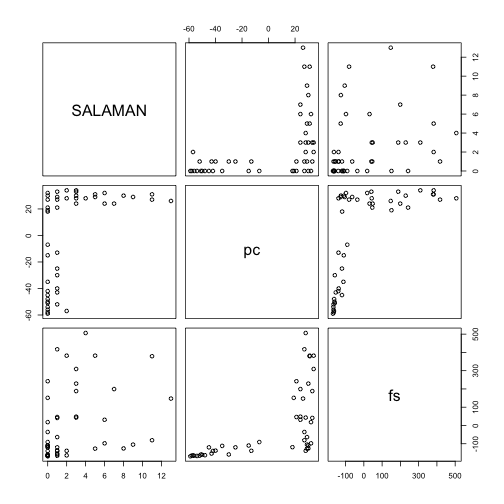
\includegraphics{notmuchinfo} \end{kframe}}
\end{knitrout}


Looking at the pairs plot, we can see perhaps why a model based on pc alone does a bad job at high counts. 
At high pc, there are counts ranging from 0 to 12 (the maximum), thus there is little information in pc to predict  at these counts. 
There are a wide range of forestage values at high percent-cover values, however, and if forestage were a strong predictor of salamander count, a model with both variables could work well. 

There's a big problem, however, with forestage as a predictor. This can be seen in the pairs plot.

\subsubsection*{(B)}

We'll see if model selection and averaging bears out our suspicion that forestage can't help much. . . 

\begin{knitrout}
\definecolor{shadecolor}{rgb}{.97, .97, .97}{\color{fgcolor}\begin{kframe}
\begin{flushleft}
\ttfamily\noindent
\hlsymbol{m2b}{\ }\hlassignement{\usebox{\hlnormalsizeboxlessthan}-}{\ }\hlfunctioncall{mle2}\hlkeyword{(}\hlsymbol{SALAMAN}{\ }\hlkeyword{\urltilda{}}{\ }\hlfunctioncall{dpois}\hlkeyword{(}\hlargument{lambda}{\ }\hlargument{=}{\ }\hlfunctioncall{exp}\hlkeyword{(}\hlsymbol{a}{\ }\hlkeyword{+}{\ }\hlsymbol{b.P}{\ }\hlkeyword{*}{\ }\hlsymbol{pc}{\ }\hlkeyword{+}{\ }\hlsymbol{b.F}{\ }\hlkeyword{*}\hspace*{\fill}\\
\hlstd{}{\ }{\ }{\ }{\ }\hlsymbol{fs}\hlkeyword{)}\hlkeyword{)}\hlkeyword{,}{\ }\hlargument{data}{\ }\hlargument{=}{\ }\hlsymbol{d}\hlkeyword{,}{\ }\hlargument{start}{\ }\hlargument{=}{\ }\hlfunctioncall{list}\hlkeyword{(}\hlargument{a}{\ }\hlargument{=}{\ }\hlfunctioncall{log}\hlkeyword{(}\hlfunctioncall{mean}\hlkeyword{(}\hlsymbol{d}\hlkeyword{\usebox{\hlnormalsizeboxdollar}}\hlsymbol{SALAMAN}\hlkeyword{)}\hlkeyword{)}\hlkeyword{,}{\ }\hlargument{b.P}{\ }\hlargument{=}{\ }\hlnumber{0}\hlkeyword{,}\hspace*{\fill}\\
\hlstd{}{\ }{\ }{\ }{\ }\hlargument{b.F}{\ }\hlargument{=}{\ }\hlnumber{0}\hlkeyword{)}\hlkeyword{)}\hspace*{\fill}\\
\hlstd{}\hlsymbol{m2c}{\ }\hlassignement{\usebox{\hlnormalsizeboxlessthan}-}{\ }\hlfunctioncall{mle2}\hlkeyword{(}\hlsymbol{SALAMAN}{\ }\hlkeyword{\urltilda{}}{\ }\hlfunctioncall{dpois}\hlkeyword{(}\hlargument{lambda}{\ }\hlargument{=}{\ }\hlfunctioncall{exp}\hlkeyword{(}\hlsymbol{a}{\ }\hlkeyword{+}{\ }\hlsymbol{b.P}{\ }\hlkeyword{*}{\ }\hlsymbol{pc}{\ }\hlkeyword{+}{\ }\hlsymbol{b.F}{\ }\hlkeyword{*}\hspace*{\fill}\\
\hlstd{}{\ }{\ }{\ }{\ }\hlsymbol{fs}{\ }\hlkeyword{+}{\ }\hlsymbol{b.PF}{\ }\hlkeyword{*}{\ }\hlsymbol{pc}{\ }\hlkeyword{*}{\ }\hlsymbol{fs}\hlkeyword{)}\hlkeyword{)}\hlkeyword{,}{\ }\hlargument{data}{\ }\hlargument{=}{\ }\hlsymbol{d}\hlkeyword{,}{\ }\hlargument{start}{\ }\hlargument{=}{\ }\hlfunctioncall{list}\hlkeyword{(}\hlargument{a}{\ }\hlargument{=}{\ }\hlfunctioncall{log}\hlkeyword{(}\hlfunctioncall{mean}\hlkeyword{(}\hlsymbol{d}\hlkeyword{\usebox{\hlnormalsizeboxdollar}}\hlsymbol{SALAMAN}\hlkeyword{)}\hlkeyword{)}\hlkeyword{,}\hspace*{\fill}\\
\hlstd{}{\ }{\ }{\ }{\ }\hlargument{b.P}{\ }\hlargument{=}{\ }\hlnumber{0}\hlkeyword{,}{\ }\hlargument{b.F}{\ }\hlargument{=}{\ }\hlnumber{0}\hlkeyword{,}{\ }\hlargument{b.PF}{\ }\hlargument{=}{\ }\hlnumber{0}\hlkeyword{)}\hlkeyword{)}\hspace*{\fill}\\
\hlstd{}\hlsymbol{m2d}{\ }\hlassignement{\usebox{\hlnormalsizeboxlessthan}-}{\ }\hlfunctioncall{mle2}\hlkeyword{(}\hlsymbol{SALAMAN}{\ }\hlkeyword{\urltilda{}}{\ }\hlfunctioncall{dpois}\hlkeyword{(}\hlargument{lambda}{\ }\hlargument{=}{\ }\hlfunctioncall{exp}\hlkeyword{(}\hlsymbol{a}{\ }\hlkeyword{+}{\ }\hlsymbol{b.F}{\ }\hlkeyword{*}{\ }\hlsymbol{fs}\hlkeyword{)}\hlkeyword{)}\hlkeyword{,}\hspace*{\fill}\\
\hlstd{}{\ }{\ }{\ }{\ }\hlargument{data}{\ }\hlargument{=}{\ }\hlsymbol{d}\hlkeyword{,}{\ }\hlargument{start}{\ }\hlargument{=}{\ }\hlfunctioncall{list}\hlkeyword{(}\hlargument{a}{\ }\hlargument{=}{\ }\hlfunctioncall{log}\hlkeyword{(}\hlfunctioncall{mean}\hlkeyword{(}\hlsymbol{d}\hlkeyword{\usebox{\hlnormalsizeboxdollar}}\hlsymbol{SALAMAN}\hlkeyword{)}\hlkeyword{)}\hlkeyword{,}{\ }\hlargument{b.F}{\ }\hlargument{=}{\ }\hlnumber{0}\hlkeyword{)}\hlkeyword{)}\hspace*{\fill}\\
\hlstd{}\hlfunctioncall{compare}\hlkeyword{(}\hlsymbol{m2a}\hlkeyword{,}{\ }\hlsymbol{m2b}\hlkeyword{,}{\ }\hlsymbol{m2c}\hlkeyword{,}{\ }\hlsymbol{m2d}\hlkeyword{,}{\ }\hlargument{nobs}{\ }\hlargument{=}{\ }\hlfunctioncall{nrow}\hlkeyword{(}\hlsymbol{d}\hlkeyword{)}\hlkeyword{)}\mbox{}
\normalfont
\end{flushleft}
\begin{verbatim}
##     k  AICc   BIC    w.AICc     w.BIC  dAICc   dBIC
## m2a 2 210.6 214.1    0.7596    0.8736  0.000  0.000
## m2b 3 212.9 217.9    0.2404    0.1264  2.301  3.866
## m2d 2 260.0 263.4 1.466e-11 1.686e-11 49.342 49.342
## m2c 4 284.2 290.7 < 2.2e-16 < 2.2e-16 73.593 76.614
\end{verbatim}
\end{kframe}}
\end{knitrout}


There is support for a model that includes both pc and fs, but with more weight on pc alone. 
(BIC and AICc agree pretty well here, so it shouldn't matter which I use)
Averaged predictions really show no difference from the predictions using pc alone. 
This is because forestage is such a poor predictor. 

\begin{knitrout}
\definecolor{shadecolor}{rgb}{.97, .97, .97}{\color{fgcolor}\begin{kframe}
\begin{flushleft}
\ttfamily\noindent
\hspace*{\fill}\\
\hlstd{}\hlsymbol{post}{\ }\hlassignement{\usebox{\hlnormalsizeboxlessthan}-}{\ }\hlfunctioncall{sample.naive.posterior}\hlkeyword{(}\hlfunctioncall{list}\hlkeyword{(}\hlsymbol{m2a}\hlkeyword{,}{\ }\hlsymbol{m2b}\hlkeyword{)}\hlkeyword{,}{\ }\hlargument{n}{\ }\hlargument{=}{\ }\hlnumber{50000}\hlkeyword{,}\hspace*{\fill}\\
\hlstd{}{\ }{\ }{\ }{\ }\hlargument{method}{\ }\hlargument{=}{\ }\hlstring{"AICc"}\hlkeyword{,}{\ }\hlargument{nobs}{\ }\hlargument{=}{\ }\hlfunctioncall{nrow}\hlkeyword{(}\hlsymbol{d}\hlkeyword{)}\hlkeyword{)}\hspace*{\fill}\\
\hlstd{}\hlsymbol{fore.mean}{\ }\hlassignement{\usebox{\hlnormalsizeboxlessthan}-}{\ }\hlfunctioncall{mean}\hlkeyword{(}\hlsymbol{d}\hlkeyword{\usebox{\hlnormalsizeboxdollar}}\hlsymbol{fs}\hlkeyword{)}\hspace*{\fill}\\
\hlstd{}\hspace*{\fill}\\
\hlstd{}\hlsymbol{y.pred}{\ }\hlassignement{\usebox{\hlnormalsizeboxlessthan}-}{\ }\hlfunctioncall{sapply}\hlkeyword{(}\hlsymbol{pct.seq}\hlkeyword{,}{\ }\hlkeyword{function}\hlkeyword{(}\hlformalargs{z}\hlkeyword{)}{\ }\hlfunctioncall{mean}\hlkeyword{(}\hlfunctioncall{exp}\hlkeyword{(}\hlsymbol{post}\hlkeyword{\usebox{\hlnormalsizeboxdollar}}\hlsymbol{a}{\ }\hlkeyword{+}{\ }\hlsymbol{post}\hlkeyword{\usebox{\hlnormalsizeboxdollar}}\hlsymbol{b.P}{\ }\hlkeyword{*}\hspace*{\fill}\\
\hlstd{}{\ }{\ }{\ }{\ }\hlsymbol{z}{\ }\hlkeyword{+}{\ }\hlsymbol{post}\hlkeyword{\usebox{\hlnormalsizeboxdollar}}\hlsymbol{b.F}{\ }\hlkeyword{*}{\ }\hlsymbol{fore.mean}\hlkeyword{)}\hlkeyword{)}\hlkeyword{)}\hspace*{\fill}\\
\hlstd{}\hspace*{\fill}\\
\hlstd{}\hlsymbol{y.pred.ci}{\ }\hlassignement{\usebox{\hlnormalsizeboxlessthan}-}{\ }\hlfunctioncall{sapply}\hlkeyword{(}\hlsymbol{pct.seq}\hlkeyword{,}{\ }\hlkeyword{function}\hlkeyword{(}\hlformalargs{z}\hlkeyword{)}{\ }\hlfunctioncall{PCI}\hlkeyword{(}\hlfunctioncall{exp}\hlkeyword{(}\hlsymbol{post}\hlkeyword{\usebox{\hlnormalsizeboxdollar}}\hlsymbol{a}{\ }\hlkeyword{+}\hspace*{\fill}\\
\hlstd{}{\ }{\ }{\ }{\ }\hlsymbol{post}\hlkeyword{\usebox{\hlnormalsizeboxdollar}}\hlsymbol{b.P}{\ }\hlkeyword{*}{\ }\hlsymbol{z}{\ }\hlkeyword{+}{\ }\hlsymbol{post}\hlkeyword{\usebox{\hlnormalsizeboxdollar}}\hlsymbol{b.F}{\ }\hlkeyword{*}{\ }\hlsymbol{fore.mean}\hlkeyword{)}\hlkeyword{)}\hlkeyword{)}\hspace*{\fill}\\
\hlstd{}\hspace*{\fill}\\
\hlstd{}\hlsymbol{y.pred.pi}{\ }\hlassignement{\usebox{\hlnormalsizeboxlessthan}-}{\ }\hlfunctioncall{sapply}\hlkeyword{(}\hlsymbol{pct.seq}\hlkeyword{,}{\ }\hlkeyword{function}\hlkeyword{(}\hlformalargs{z}\hlkeyword{)}{\ }\hlfunctioncall{PCI}\hlkeyword{(}\hlfunctioncall{rpois}\hlkeyword{(}\hlargument{n}{\ }\hlargument{=}{\ }\hlnumber{30000}\hlkeyword{,}\hspace*{\fill}\\
\hlstd{}{\ }{\ }{\ }{\ }\hlargument{lambda}{\ }\hlargument{=}{\ }\hlfunctioncall{exp}\hlkeyword{(}\hlsymbol{post}\hlkeyword{\usebox{\hlnormalsizeboxdollar}}\hlsymbol{a}{\ }\hlkeyword{+}{\ }\hlsymbol{post}\hlkeyword{\usebox{\hlnormalsizeboxdollar}}\hlsymbol{b.P}{\ }\hlkeyword{*}{\ }\hlsymbol{z}{\ }\hlkeyword{+}{\ }\hlsymbol{post}\hlkeyword{\usebox{\hlnormalsizeboxdollar}}\hlsymbol{b.F}{\ }\hlkeyword{*}{\ }\hlsymbol{fore.mean}\hlkeyword{)}\hlkeyword{)}\hlkeyword{)}\hlkeyword{)}\hspace*{\fill}\\
\hlstd{}\hspace*{\fill}\\
\hlstd{}\hspace*{\fill}\\
\hlstd{}\hlfunctioncall{plot}\hlkeyword{(}\hlsymbol{SALAMAN}{\ }\hlkeyword{\urltilda{}}{\ }\hlsymbol{pc}\hlkeyword{,}{\ }\hlargument{data}{\ }\hlargument{=}{\ }\hlsymbol{d}\hlkeyword{,}{\ }\hlargument{col}{\ }\hlargument{=}{\ }\hlfunctioncall{col.alpha}\hlkeyword{(}\hlstring{"gray"}\hlkeyword{,}{\ }\hlnumber{0.9}\hlkeyword{)}\hlkeyword{,}\hspace*{\fill}\\
\hlstd{}{\ }{\ }{\ }{\ }\hlargument{pch}{\ }\hlargument{=}{\ }\hlnumber{19}\hlkeyword{)}\hspace*{\fill}\\
\hlstd{}\hlfunctioncall{lines}\hlkeyword{(}\hlsymbol{pct.seq}\hlkeyword{,}{\ }\hlsymbol{y.pred}\hlkeyword{)}\hspace*{\fill}\\
\hlstd{}\hlfunctioncall{lines}\hlkeyword{(}\hlsymbol{pct.seq}\hlkeyword{,}{\ }\hlsymbol{y.pred.ci}\hlkeyword{[}\hlnumber{1}\hlkeyword{,}{\ }\hlkeyword{]}\hlkeyword{,}{\ }\hlargument{lty}{\ }\hlargument{=}{\ }\hlnumber{2}\hlkeyword{)}\hspace*{\fill}\\
\hlstd{}\hlfunctioncall{lines}\hlkeyword{(}\hlsymbol{pct.seq}\hlkeyword{,}{\ }\hlsymbol{y.pred.ci}\hlkeyword{[}\hlnumber{2}\hlkeyword{,}{\ }\hlkeyword{]}\hlkeyword{,}{\ }\hlargument{lty}{\ }\hlargument{=}{\ }\hlnumber{2}\hlkeyword{)}\hspace*{\fill}\\
\hlstd{}\hlfunctioncall{lines}\hlkeyword{(}\hlsymbol{pct.seq}\hlkeyword{,}{\ }\hlsymbol{y.pred.pi}\hlkeyword{[}\hlnumber{1}\hlkeyword{,}{\ }\hlkeyword{]}\hlkeyword{,}{\ }\hlargument{lty}{\ }\hlargument{=}{\ }\hlnumber{3}\hlkeyword{)}\hspace*{\fill}\\
\hlstd{}\hlfunctioncall{lines}\hlkeyword{(}\hlsymbol{pct.seq}\hlkeyword{,}{\ }\hlsymbol{y.pred.pi}\hlkeyword{[}\hlnumber{2}\hlkeyword{,}{\ }\hlkeyword{]}\hlkeyword{,}{\ }\hlargument{lty}{\ }\hlargument{=}{\ }\hlnumber{3}\hlkeyword{)}\mbox{}
\normalfont
\end{flushleft}
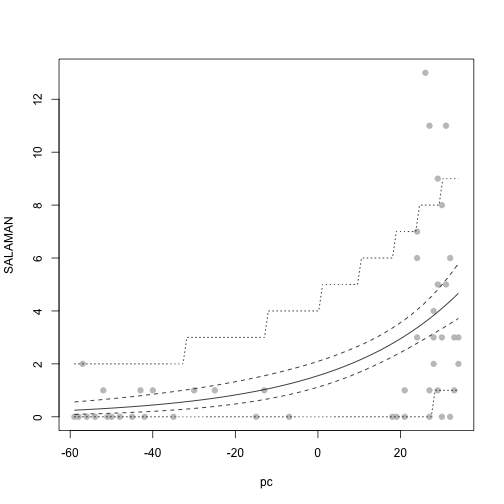
\includegraphics{2b-avg} \end{kframe}}
\end{knitrout}




\begin{knitrout}
\definecolor{shadecolor}{rgb}{.97, .97, .97}{\color{fgcolor}\begin{kframe}
\begin{flushleft}
\ttfamily\noindent
\hlsymbol{d}\hlkeyword{\usebox{\hlnormalsizeboxdollar}}\hlsymbol{cover}{\ }\hlassignement{\usebox{\hlnormalsizeboxlessthan}-}{\ }\hlfunctioncall{factor}\hlkeyword{(}\hlfunctioncall{ifelse}\hlkeyword{(}\hlsymbol{d}\hlkeyword{\usebox{\hlnormalsizeboxdollar}}\hlsymbol{pc}{\ }\hlkeyword{\usebox{\hlnormalsizeboxgreaterthan}}{\ }\hlnumber{0}\hlkeyword{,}{\ }\hlstring{"\usebox{\hlnormalsizeboxgreaterthan}{\ }60"}\hlkeyword{,}{\ }\hlstring{"{\ }\usebox{\hlnormalsizeboxlessthan}{\ }60"}\hlkeyword{)}\hlkeyword{)}\hspace*{\fill}\\
\hlstd{}\hlsymbol{g}{\ }\hlassignement{\usebox{\hlnormalsizeboxlessthan}-}{\ }\hlfunctioncall{ggplot}\hlkeyword{(}\hlsymbol{d}\hlkeyword{)}\hspace*{\fill}\\
\hlstd{}\hlsymbol{g}{\ }\hlkeyword{+}{\ }\hlfunctioncall{geom\usebox{\hlnormalsizeboxunderscore}boxplot}\hlkeyword{(}\hlfunctioncall{aes}\hlkeyword{(}\hlsymbol{cover}\hlkeyword{,}{\ }\hlsymbol{SALAMAN}\hlkeyword{)}\hlkeyword{)}{\ }\hlkeyword{+}{\ }\hlfunctioncall{geom\usebox{\hlnormalsizeboxunderscore}point}\hlkeyword{(}\hlfunctioncall{aes}\hlkeyword{(}\hlsymbol{cover}\hlkeyword{,}\hspace*{\fill}\\
\hlstd{}{\ }{\ }{\ }{\ }\hlsymbol{SALAMAN}\hlkeyword{,}{\ }\hlargument{size}{\ }\hlargument{=}{\ }\hlsymbol{FORESTAGE}\hlkeyword{)}\hlkeyword{)}\mbox{}
\normalfont
\end{flushleft}
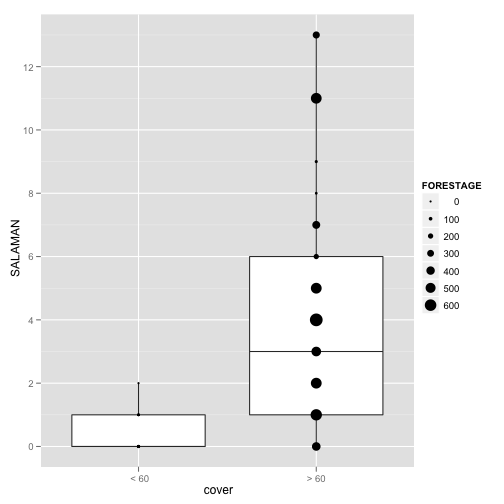
\includegraphics{cor-issue} \end{kframe}}
\end{knitrout}


Visualized another way, we see massive spread in count at high percent cover (> 60\%) and very little pattern in forestage (dot size) at these values of percent cover.

\subsection*{Colophon}

\begin{knitrout}
\definecolor{shadecolor}{rgb}{.97, .97, .97}{\color{fgcolor}\begin{kframe}
\begin{flushleft}
\ttfamily\noindent
\hlfunctioncall{require}\hlkeyword{(}\hlsymbol{knitr}\hlkeyword{)}{\ }{\ }\hlcomment{\usebox{\hlnormalsizeboxhash}\usebox{\hlnormalsizeboxhash}\usebox{\hlnormalsizeboxhash}{\ }the{\ }package}\hspace*{\fill}\\
\hlstd{}\hlfunctioncall{knit}\hlkeyword{(}\hlfunctioncall{paste}\hlkeyword{(}\hlfunctioncall{getwd}\hlkeyword{(}\hlkeyword{)}\hlkeyword{,}{\ }\hlstring{"hw7ashander.Rnw"}\hlkeyword{,}{\ }\hlargument{sep}{\ }\hlargument{=}{\ }\hlstring{"/"}\hlkeyword{)}\hlkeyword{)}{\ }{\ }\hlcomment{\usebox{\hlnormalsizeboxhash}\usebox{\hlnormalsizeboxhash}{\ }to{\ }run}\hspace*{\fill}\\
\hlstd{}\hspace*{\fill}\\
\hlstd{}\hlcomment{\usebox{\hlnormalsizeboxhash}\usebox{\hlnormalsizeboxhash}{\ }to{\ }use{\ }all{\ }cores}\hspace*{\fill}\\
\hlstd{}\hlfunctioncall{require}\hlkeyword{(}\hlsymbol{snowfall}\hlkeyword{)}\hspace*{\fill}\\
\hlstd{}\hlfunctioncall{sfInit}\hlkeyword{(}\hlargument{parallel}{\ }\hlargument{=}{\ }\hlnumber{TRUE}\hlkeyword{,}{\ }\hlargument{cpus}{\ }\hlargument{=}{\ }\hlnumber{4}\hlkeyword{)}\hspace*{\fill}\\
\hlstd{}\hlfunctioncall{sfLibrary}\hlkeyword{(}\hlsymbol{rethinking}\hlkeyword{)}\hspace*{\fill}\\
\hlstd{}\hlfunctioncall{sfExportAll}\hlkeyword{(}\hlkeyword{)}\hspace*{\fill}\\
\hlstd{}\hlfunctioncall{sfStop}\hlkeyword{(}\hlkeyword{)}\mbox{}
\normalfont
\end{flushleft}
\end{kframe}}
\end{knitrout}


\end{document}
